\chapter{A co-rotational triangular shell FEM model}
\label{chap9}
\begin{shortAbstract}
In the field of medical simulation, very few models have been proposed for simulating, in real-time, the deformation of thin anatomical structures. In fact, to our knowledge, no model based on the equations of continuum mechanics was described and applied to simulating the deformation of objects. In this chapter, we propose to rely on continuum mechanics to accurately describe the complex deformations of the implant. Our approach extends the co-rotational method used in finite element analysis of in-plane deformations to incorporate a bending energy. We will first describe the model in details before discussing its implementation in the open source framework SOFA. Lastly, this co-rotational shell FEM was applied to the simulation of the lens deployment during cataract surgery. This simulation also accounts for the complex contacts that take place during the injection phase.
\end{shortAbstract}


\section{Model description}

We propose to define a triangular shell element by combining a two-dimensional in-plane membrane energy, with an off-plane energy for describing bending and twist. To allow for real-time simulation, a computationally efficient formulation is needed. We therefore propose to extend the co-rotational idea introduced by \cite{Felippa00}. Indeed, as we have seen in the previous chapters, co-rotational approaches have been successfully applied to real-time simulation over the last few years. They offer a good trade-off between computational efficiency and accuracy by allowing small deformations but large displacements. We propose to improve and extend a plate model first introduced by \cite{Przemieniecki85} to a co-rotational formulation. Once combined with an in-plane membrane formulation we obtain an accurate, yet computationally efficient, shell finite element method featuring both membrane and bending energies. 

\subsection{Triangular elastic membrane}

The computation of the triangular elastic membrane stiffness matrix can be derived from previous works dealing with tetrahedral co-rotational elements \citep[like][for instance]{Muller04b}. The element stiffness matrix $\textbf{K}_e$ can be computed as follows:
%
\begin{equation}
\textbf{K}_e = \int_v \textbf{J} \boldsymbol\chi \textbf{J}^{T} dV,
\end{equation}
where $\textbf{J}$ is the strain-displacement matrix and $\boldsymbol\chi$ embodies the material's behaviour. The implant is very stiff and we therefore assume that the local deformations remain limited during the deployment and a linear constitutive law is sufficient. Thus in the simple case of Hooke's law we have:
%
\begin{equation}
\boldsymbol\chi = \frac{E}{12(1-\nu^2)}
\begin{bmatrix}
1 & \nu & 0 \\
\nu & 1 & 0 \\
0 & 0 & \frac{1}{2} (1-\nu)
\end{bmatrix}
\end{equation}

The stiffness matrix in the global frame is eventually obtained using the rotation matrix of the element: $\textbf{K} = \textbf{R} \textbf{K}_e \textbf{R}^{T}$ where $\textbf{R}$ describes the rotation of the (triangular) element with respect to its initial configuration.

\subsection{Triangular plate bending}

\begin{figure}[ht]
\centering
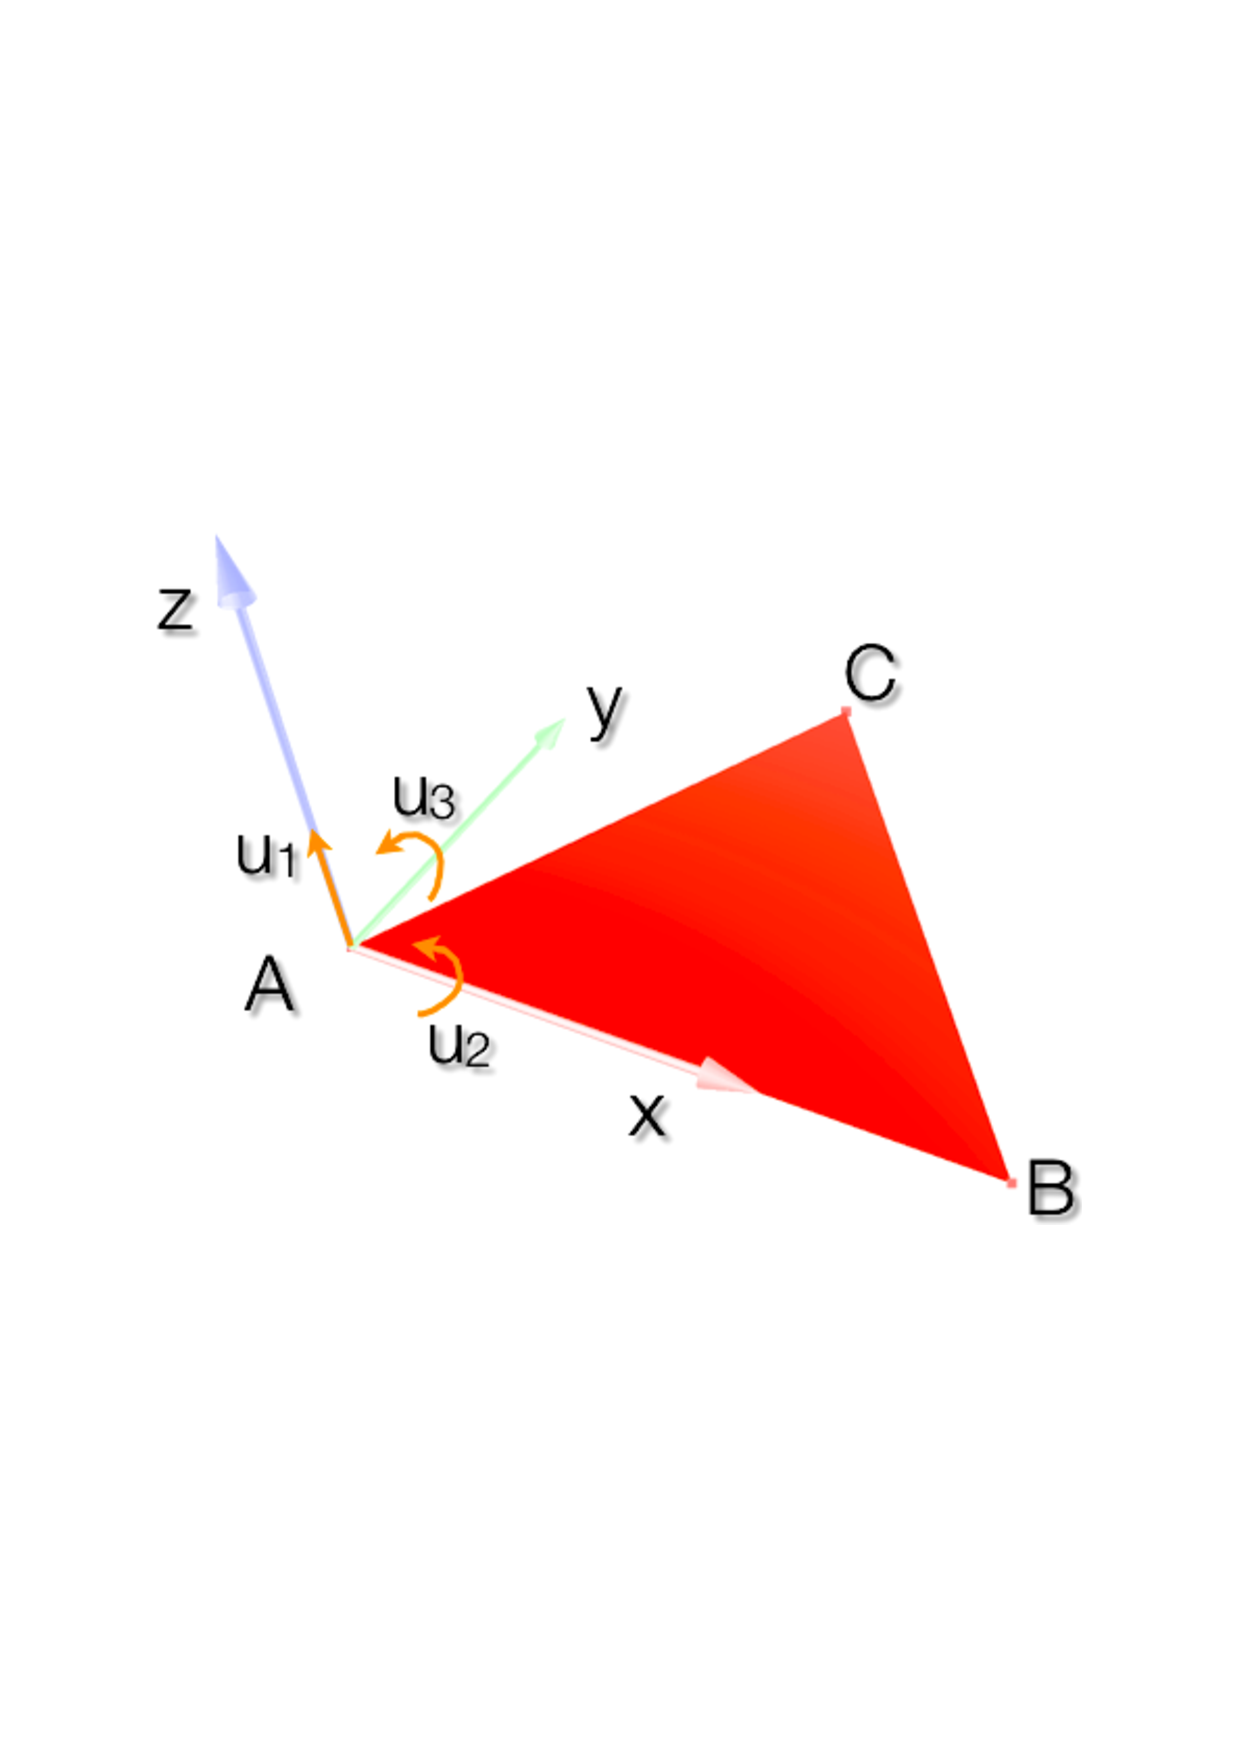
\includegraphics[height=4cm]{chapter9/bending.pdf}
\caption {The different degrees of freedom $u$ of a triangular thin plate in bending.}
\label{chap9:fig-triangle}
\end{figure}
%
To calculate the stiffness matrix for the transverse deflections and rotations shown on \fig{chap9:fig-triangle}, we start with the assumed deflection $u_z$ of the form
\begin{equation}
 u_z = c_1 + c_2x + c_3y + c_4x^2 + c_5xy + c_6y^2 + c_7x^3 + c_8xy^2 + c_9y^3,
\label{chap9:eq-deflection}
\end{equation} 
where $c_1$, \ldots , $c_9$ are constants. Equation~\ref{chap9:eq-deflection} solves an issue of symmetry which was observed with the deflection function proposed by \cite{Przemieniecki85}. These constants can be evaluated in terms of the displacements and slopes at the three corners of the triangular plate using 
\begin{equation}
\textbf{u} = \textbf{Cc}
\label{chap9:eq-U}
\end{equation} 
where $\textbf{u} = \left\{u_1 u_2 \ldots u_9 \right\} $ and $\textbf{c} = \left\{c_1 c_2 \ldots c_9 \right\} $. Matrix $\textbf{C}$ derives from \eqref{chap9:eq-U}:
\begin{equation}
C = 
	\begin{bmatrix}
	1 & 0 & 0 & 0 & 0 & 0 & 0 & 0 & 0 \\
 	0 & 0 & 1 & 0 & 0 & 0 & 0 & 0 & 0 \\
	0 & -1 & 0 & 0 & 0 & 0 & 0 & 0 & 0 \\
	1 & x_2 & 0 & x_2^2 & 0 & 0 & x_2^3 & 0 & 0 \\
	0 & 0 & 1 & 0 & x_2 & 0 & 0 & 0 & 0 \\
	0 & -1 & 0 & -2x_2 & 0 & 0 & -3x_2 & 0 & 0 \\
	1 & x_3 & y_3 & x_3^2 & x_3y_3 & y_3^2 & x_3^2 & x_3y_3^2& y_3^3 \\
	0 & 0 & 1 & 0 & x_3 & 2y_3 & 0 & 2x_3y_3 & 3y_3^2 \\
	0 & -1 & 0 & -2x_3 & -y_3 & 0 & -3x_3^2 & -y_3^2 & 0
	\end{bmatrix}
\end{equation} 

We used the following notations:
\begin{align}
u_1 &= (u_z)_{x_1,y_1}, & u_2 &= \left(\frac{\partial u_z}{\partial y}\right)_{x_1,y_1}, & u_3 &= - \left(\frac{\partial u_z}{\partial x}\right)_{x_1,y_1} \notag \\
u_4 &= (u_z)_{x_2,y_2}, & u_5 &= \left(\frac{\partial u_z}{\partial y}\right)_{x_2,y_2}, & u_6 &= - \left(\frac{\partial u_z}{\partial x}\right)_{x_2,y_2} \label{chap9:ui} \\
u_7 &= (u_z)_{x_3,y_3}, & u_8 &= \left(\frac{\partial u_z}{\partial y}\right)_{x_3,y_3}, & u_9 &= - \left(\frac{\partial u_z}{\partial x}\right)_{x_3,y_3} \notag \\
\end{align} 

\noindent We can calculate the strains from the flat-plate theory using:
\begin{equation}
e_{xx} = -z \frac{\partial^2u_z}{\partial x^2}
\end{equation} 
\begin{equation}
e_{yy} = -z \frac{\partial^2u_z}{\partial y^2}
\end{equation} 
\begin{equation}
e_{xy} = -2z \frac{\partial^2u_z}{\partial x \partial y}
\end{equation} 

\noindent Hence, using the above equations and \eqref{chap9:eq-deflection}, we have
\begin{equation}
\begin{bmatrix}
e_{xx} \\
e_{yy} \\
e_{xy}
\end{bmatrix}
= 
-z
\begin{bmatrix}
0 & 0 & 0 & 2 & 0 & 0 & 6x & 0 & 0 \\
0 & 0 & 0 & 0 & 0 & 2 & 0 & 2x & 6y \\
0 & 0 & 0 & 0 & 2 & 0 & 0 & 4y & 0 \\
\end{bmatrix}
\textbf{c}
\label{chap9:eq-strains}
\end{equation} 
or symbolically $\textbf{e} = \textbf{Dc}$ where $\textbf{D}$ stands for the $3\times 9$ matrix in \eqref{chap9:eq-strains}, including the pre-multiplying constant $-z$. Noting from \eqref{chap9:eq-U} that $\textbf{c} = \textbf{C}^{-1}\textbf{u}$, we have:
\begin{equation}
\textbf{e} = \textbf{DC}^{-1}\textbf{u} = \textbf{bu},
\end{equation} 
where $\textbf{b} = \textbf{DC}^{-1}$. 

\noindent Knowing that the stiffness matrix $\textbf{K}_e$ for an element is obtained from
\begin{equation}
\textbf{K}_e = \int_v \textbf{b}^{T} \boldsymbol\chi \textbf{b} dV,
\end{equation} 
where $\boldsymbol\chi$ is the material matrix, the substitution of $\textbf{b}$ into this expression yields
\begin{equation}
\label{chap9:Ke}
\textbf{K}_e = (\textbf{C}^{-1})^T \int_v \textbf{D}^{T} \boldsymbol\chi \textbf{D} dV \, \textbf{C}^{-1}.
\end{equation} 

Similarly to the membrane stiffness matrix, the bending stiffness matrix in the global frame is eventually obtained using the rotation matrix of the element: $\textbf{K} = \textbf{R} \textbf{K}_e \textbf{R}^{T}$. While the method to numerically compute the integral will be reviewed section \ref{chap9:numericalIntegration}, we first carry on with the theory by introducing how the contacts are handled.  


\section{Mechanical interactions with the curved surface of shells}	\label{chap9:interactions}

The practical interest of modelling complex behaviours such as bending and twisting would remain fairly low for medical simulation if contacts and constraints were not handled properly. In our case the difficulty comes from different sources. First the collision detection must be carried out with the curved surface of shell elements as opposed to the classic detection on plane triangles. Then forces applied to a given triangle need to be distributed between linear forces and torques onto its three vertices. As we will see, the same polynomial interpolation function chosen to compute the bending energy in our FEM formulation is also used to capture the interactions between the curved surface and other objects. 

In order to detect the collision with the bent surface, we have chosen the subdivision approach. We first sample the flat surface of each element by recursively dividing each triangle into four smaller ones and the deflection of each new vertex is computed using \eqref{chap9:eq-deflection} according to the displacements and slopes at the three vertices of the triangular element. This process of subdivision may also allow us to render each shell as a curved triangle (\fig{chap9:fig-shell} (a) and (b)) and detect any collision with the curved surface of the shell using any of the classic collision detection algorithms working on flat triangles.

Once a collision has been detected, it must be processed by distributing the linear force received on the bent surface between the three vertices of the triangle. First the linear part of the force is simply transmitted on each node using the barycentric coordinates of the contact point's projection onto the triangle. 

The main difficulty is to convert the normal component of the force applied to the bent surface into a torque at each of the three nodes (\fig{chap9:fig-shell} (c)). Our approach is the following: during force computation, we use the change in orientation measured at each node to compute the local deflection of each subvertex within the triangle. Differentiating the formulation twice yields a relation between the torque applied at each node and the generated force in bending. We therefore need to invert the latter formulation to convert a bending force into torques at each vertex. Thus, we are able to transmit any force coming from interactions with the curved surface of shells to the mechanical vertices used in our FEM formulation. 
%
\begin{figure}[ht]
\centering
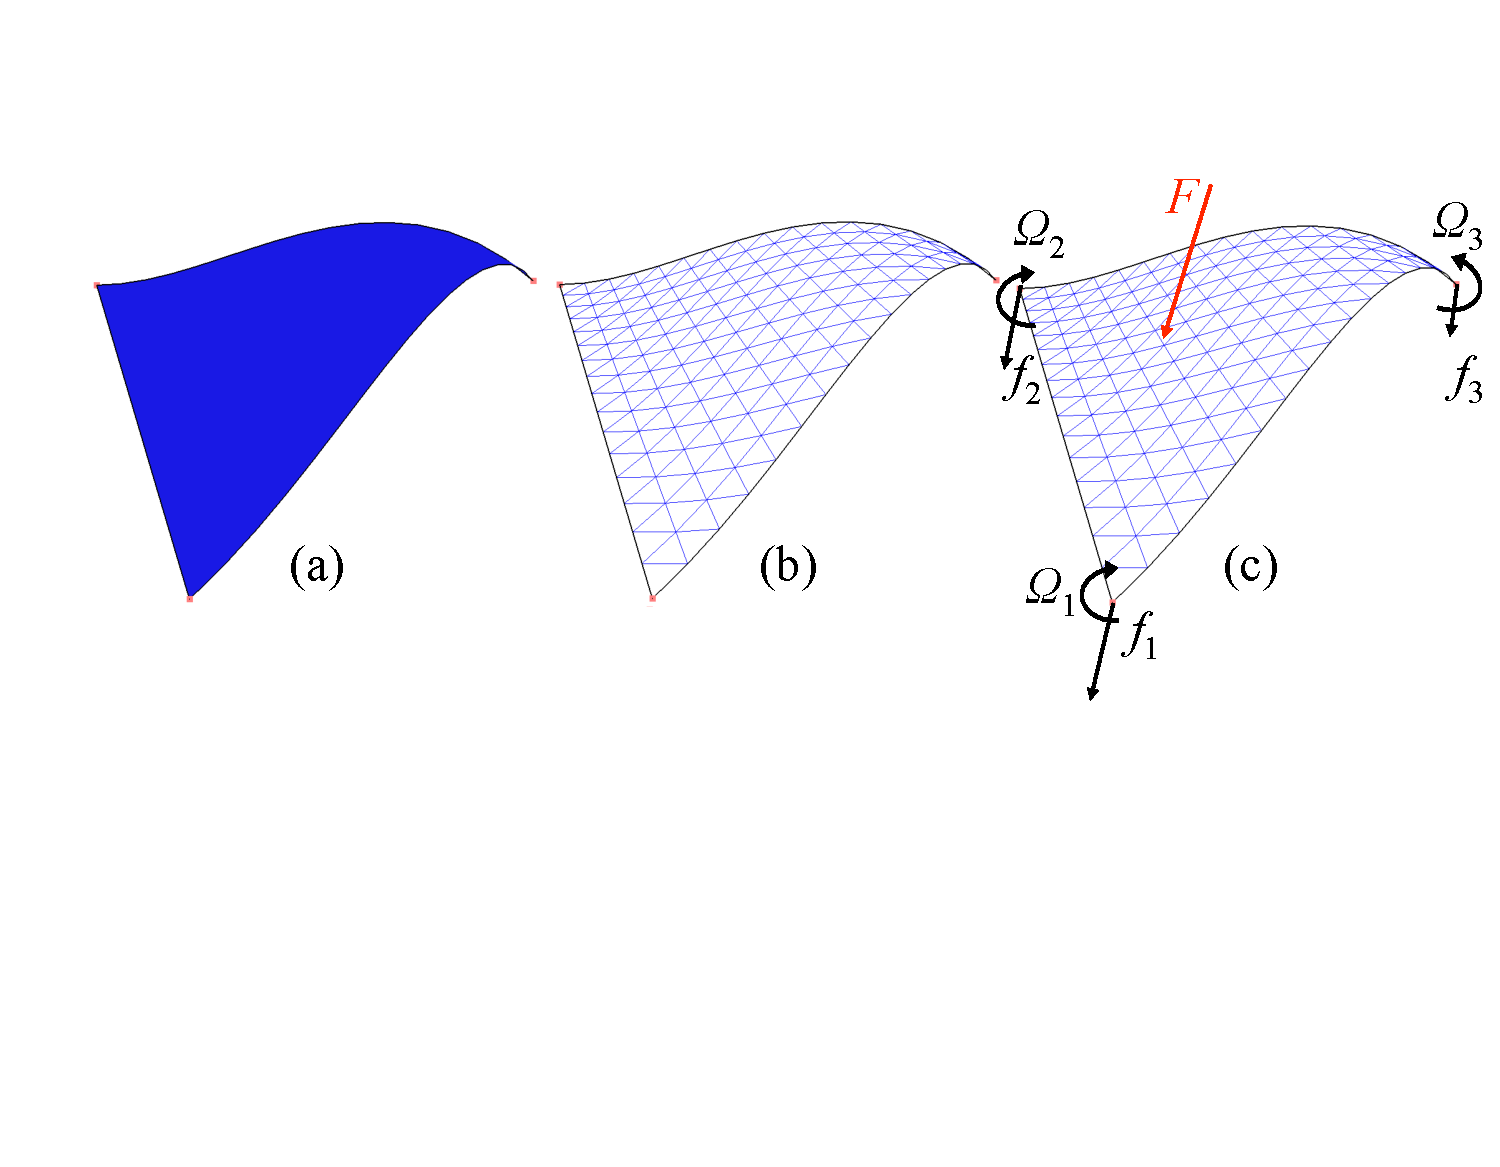
\includegraphics[width=12cm]{chapter9/shell_curvature.pdf}
\caption {(a)  The triangle formed by the three vertices of the shell has been recursively subdivided 3 times and the deflection of each new vertex was computed according to the same deflection function used in our shell FEM. (b) Sampling the actual surface of the shell allows more accurate rendering and collision detection. (c) The shape function is used to distribute an external force $F$ onto the triangle nodes.}
\label{chap9:fig-shell}
\end{figure}


\section{Implementation}

The co-rotational shell formulation has been successfully implemented as a Force Field component into the open-source framework SOFA \citep{Allard07}. A description of SOFA's architecture was given in section \ref{chap6:SOFA}. We will now review the key points of the implementation.

	\subsection{Evaluation of displacements}
The computation of the stiffness matrix, and subsequently the internal forces, starts with the measure of the displacements $\left\{u_1 u_2 \ldots u_9 \right\} $ for every element. As defined by \eqref{chap9:ui}, we need to measure the displacement along the z axis and the rotations around local x and y axes for each vertex. For \cite{Przemieniecki85}, the deflection z is measured in the global frame. But in a co-rotational formulation, a local frame is attached to each triangle and used to compute displacements and forces. In this local frame (formed from the 3 vertices) the deflection is therefore always null (hence, $ u_1, u_4, u_7 $ are null). To evaluate the remaining rotations, we first associate a quaternion at each vertex which embodies its frame (or its orientation). In mathematics, quaternions are an extension of complex numbers and may be written as follows:
\begin{equation}
q = w + x i + y j + z k \quad \mbox{with } i^2 = j^2 = k^2 = -1.
\end{equation}
For use in geometry, quaternions are often written as a sum of a scalar and a vector:
\begin{equation}
q = w + (x, y, z) = \cos (\frac{\alpha}{2}) + \mathbf{u} \sin (\frac{\alpha}{2}),
\end{equation}
where $ \mathbf{u} $ is a unit vector and $ \alpha $ a scalar. If we denote by $ \mathbf{v} $ a vector in $\field{R}^3$, it can be shown that the quaternion product $ q \mathbf{v} q^{-1} $ yields a vector which is the rotation of $ \mathbf{v} $ by an angle $ \alpha $ around the axis $ \mathbf{u} $. Quaternions require less storage than rotation matrices and are known to be more numerically stable. 

From there, our approach to measure the rotations around local x and y axes is simple. At runtime and for each vertex, we compute the rotation that we need to transform the z axis of the triangle's frame into the z axis of the vertex's frame. The differences with the same quantities computed for the rest position during the initialisation lead to the desired displacements. 
% (see listing \ref{chap9:qDiffZ})
%\begin{lstlisting}[caption={[Method to compute the rotation between two quaternions]Method used to compute the rotation of the z axis between the frames embodied by two quaternions},label={chap9:qDiffZ},frame=shadowbox,rulesepcolor=\color{black}]
%inline Quat qDiffZ(const Quat& Qvertex, const Quat& Qtriangle)
%{
%    // dQ is the quaternion that embodies the rotation between 
%    // the z axis of the vertex and the z axis of the local 
%    // triangle's frame (in local space)
%    Quat dQ;
%
%    // u = z axis of the triangle's frame (in local space)
%    Vec3d u(0,0,1);
%
%    // v = z axis of the vertex's frame is expressed into 
%    // world space
%    Vec3d v = Qvertex.rotate(Vec3d(0.0, 0.0, 1.0));
%    
%    // v0 = v expressed into local triangle's frame
%    Vec3d v0 = Qtriangle.rotate(v);
%
%    // Axis of rotation between the 2 vectors u and v lies 
%    // into the plan of the 2 vectors
%    Vec3d axis = cross(u, v0);
%    
%    // Shortest angle between the 2 vectors
%    double angle = acos(dot(u, v0));
%
%    // Quaternion associated to this axis and this angle
%    if (fabs(angle)>1e-6)
%    {
%        dQ.axisToQuat(axis,angle);
%    }
%    else
%    {
%        dQ = Quat(0,0,0,1);
%    }
%
%    return dQ;
%}
%\end{lstlisting}


%	\subsection{Inversion of matrix $ \mathbf{C} $}
%\cite{Przemieniecki85} described the condition of non-inversion for the matrix $\mathbf{C}$ as the following:
%\TODO{add condition of inversion... but need the book :)}
%
%Each triangle of a mesh obtained from a regular grid of points fits this condition of non-inversion (right triangles). We fixed this limitation by choosing a different local coordinate system that the one introduced by \citeauthor{Przemieniecki85}. 
%
%\TODO{add figure with the two different coordinate system}


	\subsection{Numerical integration} \label{chap9:numericalIntegration}
In practice, the integration of the integral in \eqref{chap9:Ke} must be carried out numerically using Gaussian quadrature, a numerical technique which allows to calculate the value of an integral. The Gaussian quadrature states that the integral of a function $ f $ over the area $ A $ of a triangular surface may be evaluated as a weighted sum of function values at specific points within the area of integration \citep{Cowper73}. In other words, we have
\begin{equation}
\int_{A} f dA = A \sum_{i=1}^n w_i f_i,
\end{equation}
where $ w_i $ is a weight factor and $ f_i $ is the evaluation of $ f $ at the integration point $ i $ (also called Gauss points). The choice of the number and the locations of the integration points depends on the order of accuracy desired. We classically choose 3 integration points located at the middle of each edge of the triangle, for which the weight factors $ w_i $ are $ 1/3 $. The required integration over the volume is achieved by multiplying the result by the thickness $ t $ of the shell. Therefore, \eqref{chap9:Ke} may be numerically evaluated as
\begin{equation}
\textbf{K}_e = \dfrac{A t}{3} (\textbf{C}^{-1})^T \sum_{i=1}^3 \textbf{D}_i^{T} \boldsymbol\chi \textbf{D}_i  \, \textbf{C}^{-1},
\end{equation}
where $ D_i $ is the evaluation of the matrix $ \mathbf{D} $ defined by \eqref{chap9:eq-strains} at each Gauss point $ i $. 

\bigskip

\subsection{Computation of stiffness matrix: summary}	\label{chap9:summary}
In practical terms, the different computations associated with each triangular shell element can be described as follows:
%
\begin{enumerate}
\item Compute the rotation matrix $\textbf{R}$ from global to triangle (local) frame
\item Compute the local displacement vector $\textbf{u} = \{v_1, v_2, 0, u_2, u_3, v_3, v_4, 0, u_5, u_6,$ $v_5, v_6, 0, u_8, u_9 \} $ for each triangle, where $ (v_1, v_2), (v_3, v_4) and (v_5, v_6) $ are the in-plane displacements on x and y local axes and $ u_i $ were defined by \eqref{chap9:ui}. As we are in a co-rotational framework, we recall that the normal displacements $u_1, u_4, u_7$ at each of the three nodes are null in the local frame of the triangle. 
\item Compute matrix $\textbf{D}_i$  at each Gauss point $i$
\item The strain-displacement matrix at each Gauss point $i$ is computed with $\textbf{J}_i = \textbf{D}_i \textbf{C}^{-1}$
\item Compute the local stiffness matrix $\textbf{K}_e$ of the element as $\textbf{K}_e = \displaystyle{\sum^3_{i=1}} \textbf{J}_i \boldsymbol\chi \textbf{J}_i^T$
\item Transform the local element stiffness matrix into the global frame and add it to the global stiffness matrix
\end{enumerate}


	\subsection{Concept of mappings in SOFA}	\label{chap9:mappings}
Let us explain the concept of \emph{mappings} and \emph{mechanical mappings} in SOFA. In SOFA, the state of a simulated system can be described by the values and time derivatives of its independent degrees of freedom (DOF) gathered in two vectors $x_0$ and $v_0$. Geometry can be attached to the DOF for visualisation or contact computation. We call it the \emph{shape}. It is typically defined by points, such as triangle vertices or sphere centers, and additional data such as triangle connectivity or sphere radii. We call these points the vertices. Their positions, velocities and associated forces are stored in vectors $x_1$ , $v_1$ and $f_1$, respectively. They are not independent variables, since the positions and velocities are bound to the DOF using kinematic operators which we call the \emph{mappings}:
\begin{eqnarray*}
x_1 &=&\JNL_1(x_0)\\ 
v_1 &=& J_1 v_0
\end{eqnarray*}
When the vertices and the DOF are the same, the mapping is the identity. Matrix $J_1 = \frac{\partial x_1}{\partial x_0}$ encodes the linear relation between the DOF velocities and the shape velocities. Due to linearity, the same relation holds on elementary displacements $dx$. It also holds on accelerations, with an additional offset due to velocities when the position mapping \JNL is non-linear. In most cases, operators \JNL~ and \J~ are the same, but in the case of rigid bodies, \JNL~ is nonlinear with respect to $x$ and it can not be written as a matrix.

When shapes collide, additional geometry can be necessary to model the contact. For instance, when an edge intersects another one, a contact force is applied to the intersection points. These points are defined by their barycentric coordinates with respect to their edge vertices. Other relations can be used, depending on the kind of geometrical primitives in contact. This additional geometry requires another geometrical layer connected to the shape by a mapping, as illustrated in \fig{chap9:fig-mappings}.

\begin{figure}[ht]
	\begin{center}
 		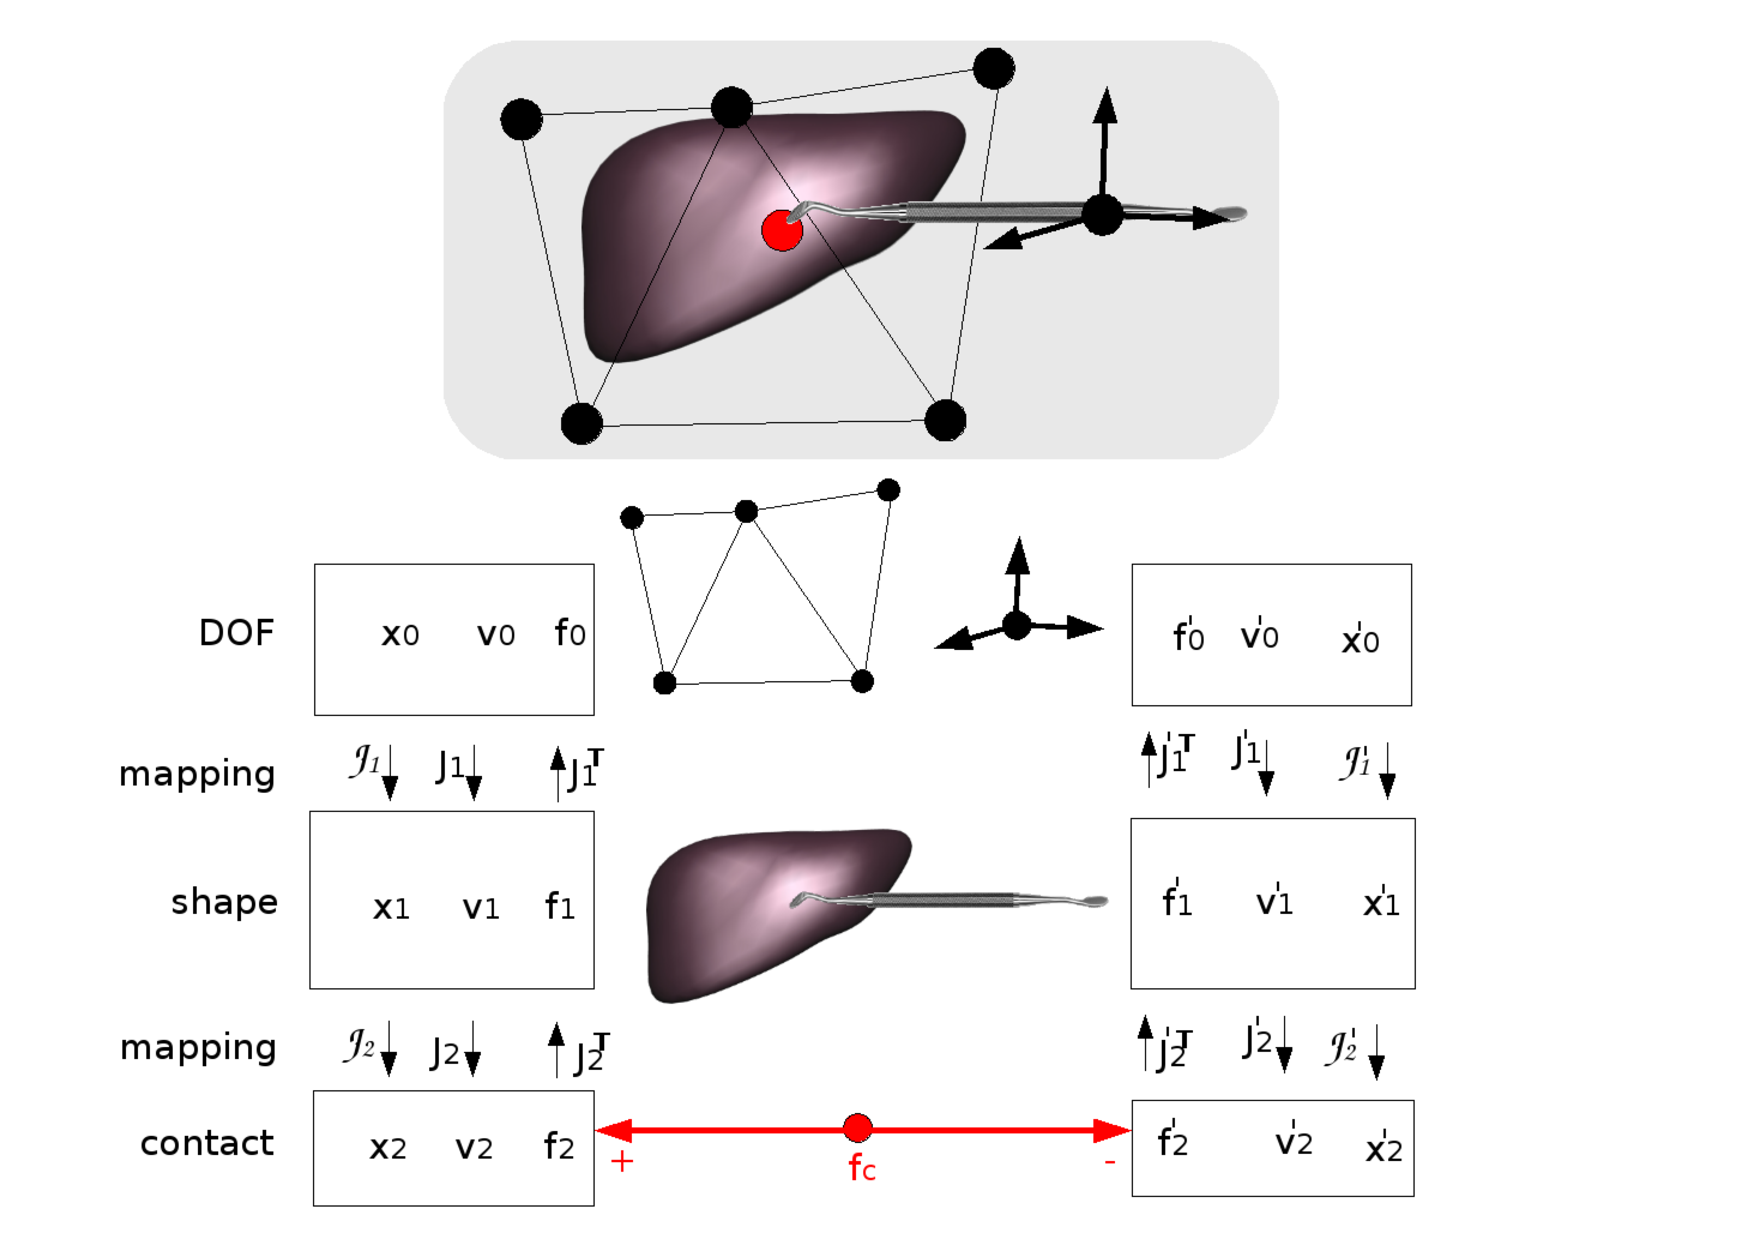
\includegraphics[width=13cm]{chapter9/mappings}
 	\end{center}
 \caption[Concept of mappings in SOFA]{Mappings from the DOFs to a contact point. Top: two simulated objects in contact (red point). Bottom: hierarchy of geometrical layers. Positions and velocities are propagated top-down. The contact force $f_c$ is accumulated in the contact layers. Forces are then propagated bottom-up. Image courtesy of SOFA's documentation. }
\label{chap9:fig-mappings}
\end{figure}

Positions and velocities can be propagated top-down through our layer hierarchy using the relations presented. In order to take the contact forces into account in the dynamics equation, we have to convert the contact forces applied to the contact points to forces applied to the DOF, where our mechanical model is applied. This requires an extension to the position and velocity mappings presented: we call it \emph{mechanical mapping}. This is a general method to propagate forces bottom-up through the layers of the geometrical hierarchy. Given forces $f_n$ applied to a geometry layer $n$, we derive the equivalent force applied to its parent layer $n-1$. Equivalent forces must have the same power. Thus, we have to compute $f_{n-1}$ such that:
$$
v_{n-1}^T f_{n-1} = v_n^T f_n
$$
The relation $v_{n} = J_{n}v_{n-1}$ allows us to rewrite the previous equation as
$$
v_{n-1}^T f_{n-1} = v_{n-1}^T J_{n}^T f_n
$$
Since this relation must hold for any velocity $v_{n-1}$, we simplify it and get
\begin{equation} \label{eq:mapF}
f_{n-1} = J_n^T f_n
\end{equation}
This corresponds to the principle of virtual work.


\subsection{Visualisation}
Because shells have a curved surface, a specific rendering technique is required to visualise the deformation in bending. Without any consideration, the shells would appear flat (as simple triangles). Our idea is to make use of a higher resolution mesh whose deformation would be controlled by the underlying physical mesh of shells. In other words, a mapping was implemented to connect the DOFs of our mechanical model to a set of vertices useful for rendering. In SOFA, a mapping has only 2 methods: init(), which allows computations during the initialisation phase, and apply() called at runtime and in charge of updating the positions of the high resolution mesh according to the coarser mesh constituted by the shell elements. 

\begin{itemize}
\item \textbf{init()} \\
During the initialisation phase, each vertex from the high resolution mesh is projected onto the coarse mesh. Thus, for each vertex we find the closest primitive (DOF, edge or triangle) on the coarse mesh and we take the list of triangles attached to it. Then, the barycentric coordinates of the projected point is computed within each triangle of this list.
%
\item \textbf{apply()} deals with the relation between the DOFs and the vertices used for rendering (shape vertices). The position of each vertex from the high resolution mesh must be updated according to the underlying mesh. After the initialisation phase, we have associated each rendering vertex to a triangle and its barycentric coordinates within this triangle are known. Therefore, we first start by computing the new position of the rendering vertex by weighting the coordinates of each triangle's vertex with the associated barycentric weight. Hence, we obtain a new position in the plane of the triangle. If we were to stop the procedure here, the shell elements would still be rendered as flat triangles since all rendering vertex are located in the plane of the triangles. Consequently, the additional step of computing the deflection is required. We know that the deflection at any point of local coordinates $(x, y)$ may be computed from $u_z = c_1 + c_2x + c_3y + c_4x^2 + c_5xy + c_6y^2 + c_7x^3 + c_8xy^2 + c_9y^3$ as described by \eqref{chap9:eq-deflection}. Hence, we calculate the local coordinates $(x, y)$ of each rendering vertex within its associated triangle. Moreover, we notice that the coefficients $ \mathbf{c} = \left\{c_1 c_2 \ldots c_9 \right\} $ may be evaluated using \eqref{chap9:eq-U} from
\begin{equation}
\mathbf{c} = \mathbf{C}^{-1} \mathbf{u},
\end{equation}
The deflection may therefore be computed for each vertex and added to the in-plane position previously calculated. 
\end{itemize}

It is worth noting that a high resolution mesh may be obtained by recursively subdividing each triangle. However, in this case the vertices are closely related to the structure of the mechanical mesh and rendering artifacts may appear. As we can notice on \fig{chap9:fig-rendering}, the quality of the visualisation may be improved by using a totally different mesh.
%
\begin{figure}[ht]
\centering 
\subfloat[Subdivided triangles]{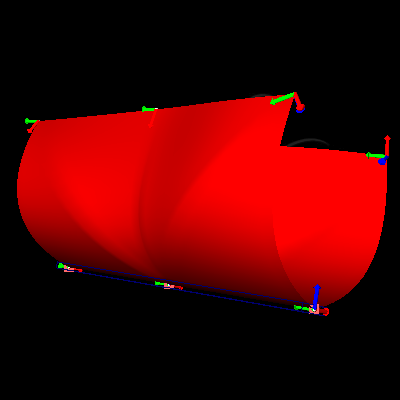
\includegraphics[width=5.5cm]{chapter9/sub_grid_red.png}}
\hspace{1cm}
\subfloat[Irregular grid]{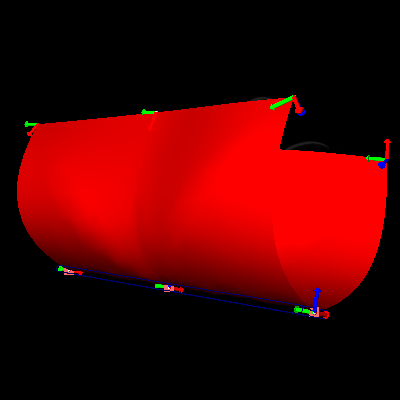
\includegraphics[width=5.5cm]{chapter9/irregular_grid_red.png}} \\
\subfloat[Subdivided triangles]{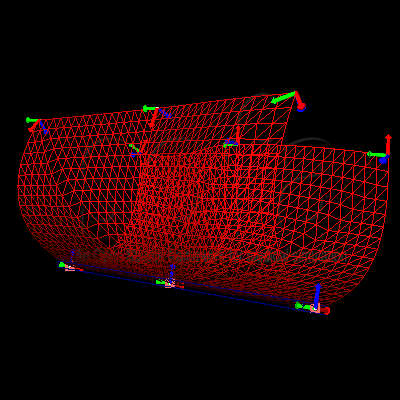
\includegraphics[width=5.5cm]{chapter9/sub_grid_mesh.png}}
\hspace{1cm}
\subfloat[Irregular grid]{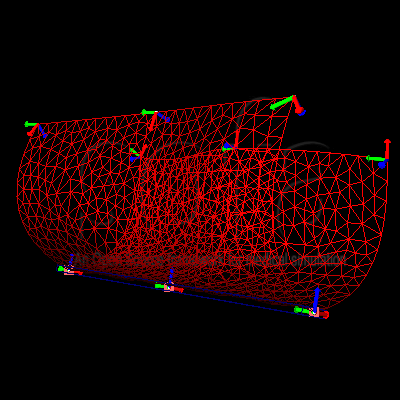
\includegraphics[width=5.5cm]{chapter9/irregular_grid_mesh.png}}
\caption[Visual artifacts using triangle subdivisions]{In some situations, some rendering artifacts may appear when we use subdivided triangles to render the shells (a,c). Using an irregular mesh which is not closely related to the structure of the mechanical mesh reduces the impact (b,d).}
\label{chap9:fig-rendering}
\end{figure}


	\subsection{Contacts with the curved surface of shells}
If a specific rendering technique was developed to visualise the curved shape of the shells, it is also essential to interact with it. Indeed, as explained section \ref{chap9:interactions}, the force applied onto the curved surface of the shell must be processed by distributing the linear force received on the bent surface between the three vertices of the triangle. Consequently, the mapping previously described is extended to a mechanical mapping and two additional methods need to be implemented: applyJ and applyJT. 
%
\begin{itemize}
\item \textbf{applyJ()} encodes the linear relation between the DOF velocities and the shape velocities as described in section \ref{chap9:mappings}. applyJ() basically embodies the same computations than apply() except that the vector of displacement $\mathbf{u}$ is different. Whereas the local displacement in rotation is measured from the quaternions to create the vector $\mathbf{u}$, this time the vector is directly obtained from the angular velocities we had at each vertex (once converted into the local frame). We therefore have a relation between the angular velocities at each vertex and the velocity of the deflection in the direction normal to each triangle. 
\item \textbf{applyJT()} must convert the contact forces applied to the contact points to forces applied to the DOF. If the linear forces are easily distributed between DOFs using barycentric coordinates, it also encodes the relation between the vertical force $ \mathbf{F} $ applied onto the bent surface of the plate and the torque at each DOF. We start by retrieving the normal component of the applied force vector $F_{\mathrm{z}}$. We project the application point of the force into the triangle's plane and compute its local coordinates $(x,y)$. We create the polynom $P$ such as 
%
\begin{equation}
P = F_{\mathrm{z}}(1 \hspace{0.2cm} x \hspace{0.2cm} y \hspace{0.2cm} x^2 \hspace{0.2cm} xy \hspace{0.2cm} y^2 \hspace{0.2cm} x^3 \hspace{0.2cm} xy^2 \hspace{0.2cm} y^3)^T. 
\end{equation}
%
The moments at each vertex are then obtained with 
\begin{equation}
\Omega = (\textbf{C}^{-1})^T P.
\end{equation}
\end{itemize}


\subsection{Allowing a curved rest configuration}
In \cite{Przemieniecki85}, the rest and initial configurations are both assumed to be the flat one. The only way to have an initial deformed shape is to apply a torque on the vertices of the shells. However, in this configuration we would compute a displacement vector $ \mathbf{u} $ that is not null, which leads to a bending energy. In order to define a curved rest configuration for our shells, we propose to compute the bending energy between the initial and rest configuration during the initialisation phase, and add the energy between the current and initial configurations at runtime. Consequently, by separating initial and rest configurations, it is possible to have an initial deformed shape without any initial bending energy. In other words, we shifted the zero energy configuration.


\subsection{Possible extension: parallel implementation on GPU}	\label{chap9:GPU}
If we look closely at all the steps required to compute the local stiffness matrix for each element (see section \ref{chap9:summary} for a summary), we can notice that the operations carried out for a given shell element are independent of the other elements. This feature makes our co-rotational shell FEM implementation highly parallelisable. One potential problem however, is the assembly of the global stiffness matrix. Indeed, in a parallel implementation, many elements are processed concurrently (that is, at the same time). Inevitably, two elements sharing a node may be processed in the same time. Therefore, they may try to both write their element contribution into the exact same location in the global stiffness matrix, and therefore the same location in GPU's memory. As with the TLED implementation described in chapter \ref{chap6}, there is two solutions. The first one would be to re-order the elements organisation so that no concurrent writes will occur. Unfortunately, this re-organisation of the element reduces the number of elements that can be processed in parallel. The second solution would be to take advantage of a new GPU NVIDIA architecture called Fermi, which added the capability atomic writes for floats. We recall that the write operation is said to be atomic in the sense that it is guaranteed to be performed without interference from other threads. In other words, the concurrent writes are simply serialised in hardware. Obviously, an additional overhead is to be expected. 

Moreover, because shells are high-order (curved) elements, fewer elements are needed to describe a given geometry with the same precision (as compared to using flat triangles). Generally speaking, this constitutes a decisive computational advantage since fewer elements are required. However, GPUs are more efficient when they tackle numerous but simple computations. Hence, a good speedup over sequential CPU implementations is usually only achieved when the number of elements involved becomes great enough. In contrast, the computations for each shell element are quite heavy and the number of elements used in the whole simulation is limited. Therefore, the conditions are not optimal to obtain maximum speedups on GPU. A straightforward GPU implementation of our shell FEM formulation where each thread deals with the calculations of one element would not make use of all the GPU capacity (the occupancy would not be maximal). If a reasonable improvement over the CPU implementation will probably be obtained nevertheless, the gain is likely to be smaller than in the case of the TLED algorithm for instance. Other approaches will need to be investigated to take full advantage of the GPU. For instance, computations within an element could be distributed between several threads to increase the occupancy of the GPU and hence the overall efficiency. 

To conclude on a possible parallelisation of the algorithm, an optimal GPU implementation is always a challenge to achieve. One needs to choose wisely the type of memory to be used for each variable and optimise the access patterns. While it seems that there is no major obstacle for a simple GPU implementation, the best speedups will only be attained through more elaborate techniques of parallelisation making full usage of the GPU. Although it will take some time, our co-rotation shell FEM will eventually be ported to GPU. 


\section{Comparison with an analytical result}

We compared our model with some theoretical results reported by \cite{Zhongnian86} to assess its quality in modelling bending. The test that we carried out uses a square shape mesh clamped on all four edges. A uniform load is then applied on the square and the maximum deflection $z_{max}$ at the centre can be calculated. Several simulations are performed with increasing load values $q$ (ranging from $1$ to 5 N/m$^2$) and the following parameters were used: 
\begin{itemize}
 \item Young Modulus $E = 1.092 \times 10^6\,$Pa
 \item Poisson's ratio $\nu = 0.3$
 \item edge of the square $L = 10\,$m
 \item thickness $h = 0.1\,$m
 \item pressure q is a uniformly distributed load per unit area
\end{itemize}

Using these particular values it can be shown that $z_{max} = 0.126\,q$. The maximum deflection obtained in our simulations are reported in Table~\ref{chap9:tab-results}. In average we found $z_{max} = 0.1248\,q $, resulting in a $0.93\,\%$ error between our model and theoretical results on that test. 
%
\begin{table}[ht]
	\centering
	\begin{tabular}{p{9cm}|c|c|}
	\cline{2-3}
	\multirow{5}{*}{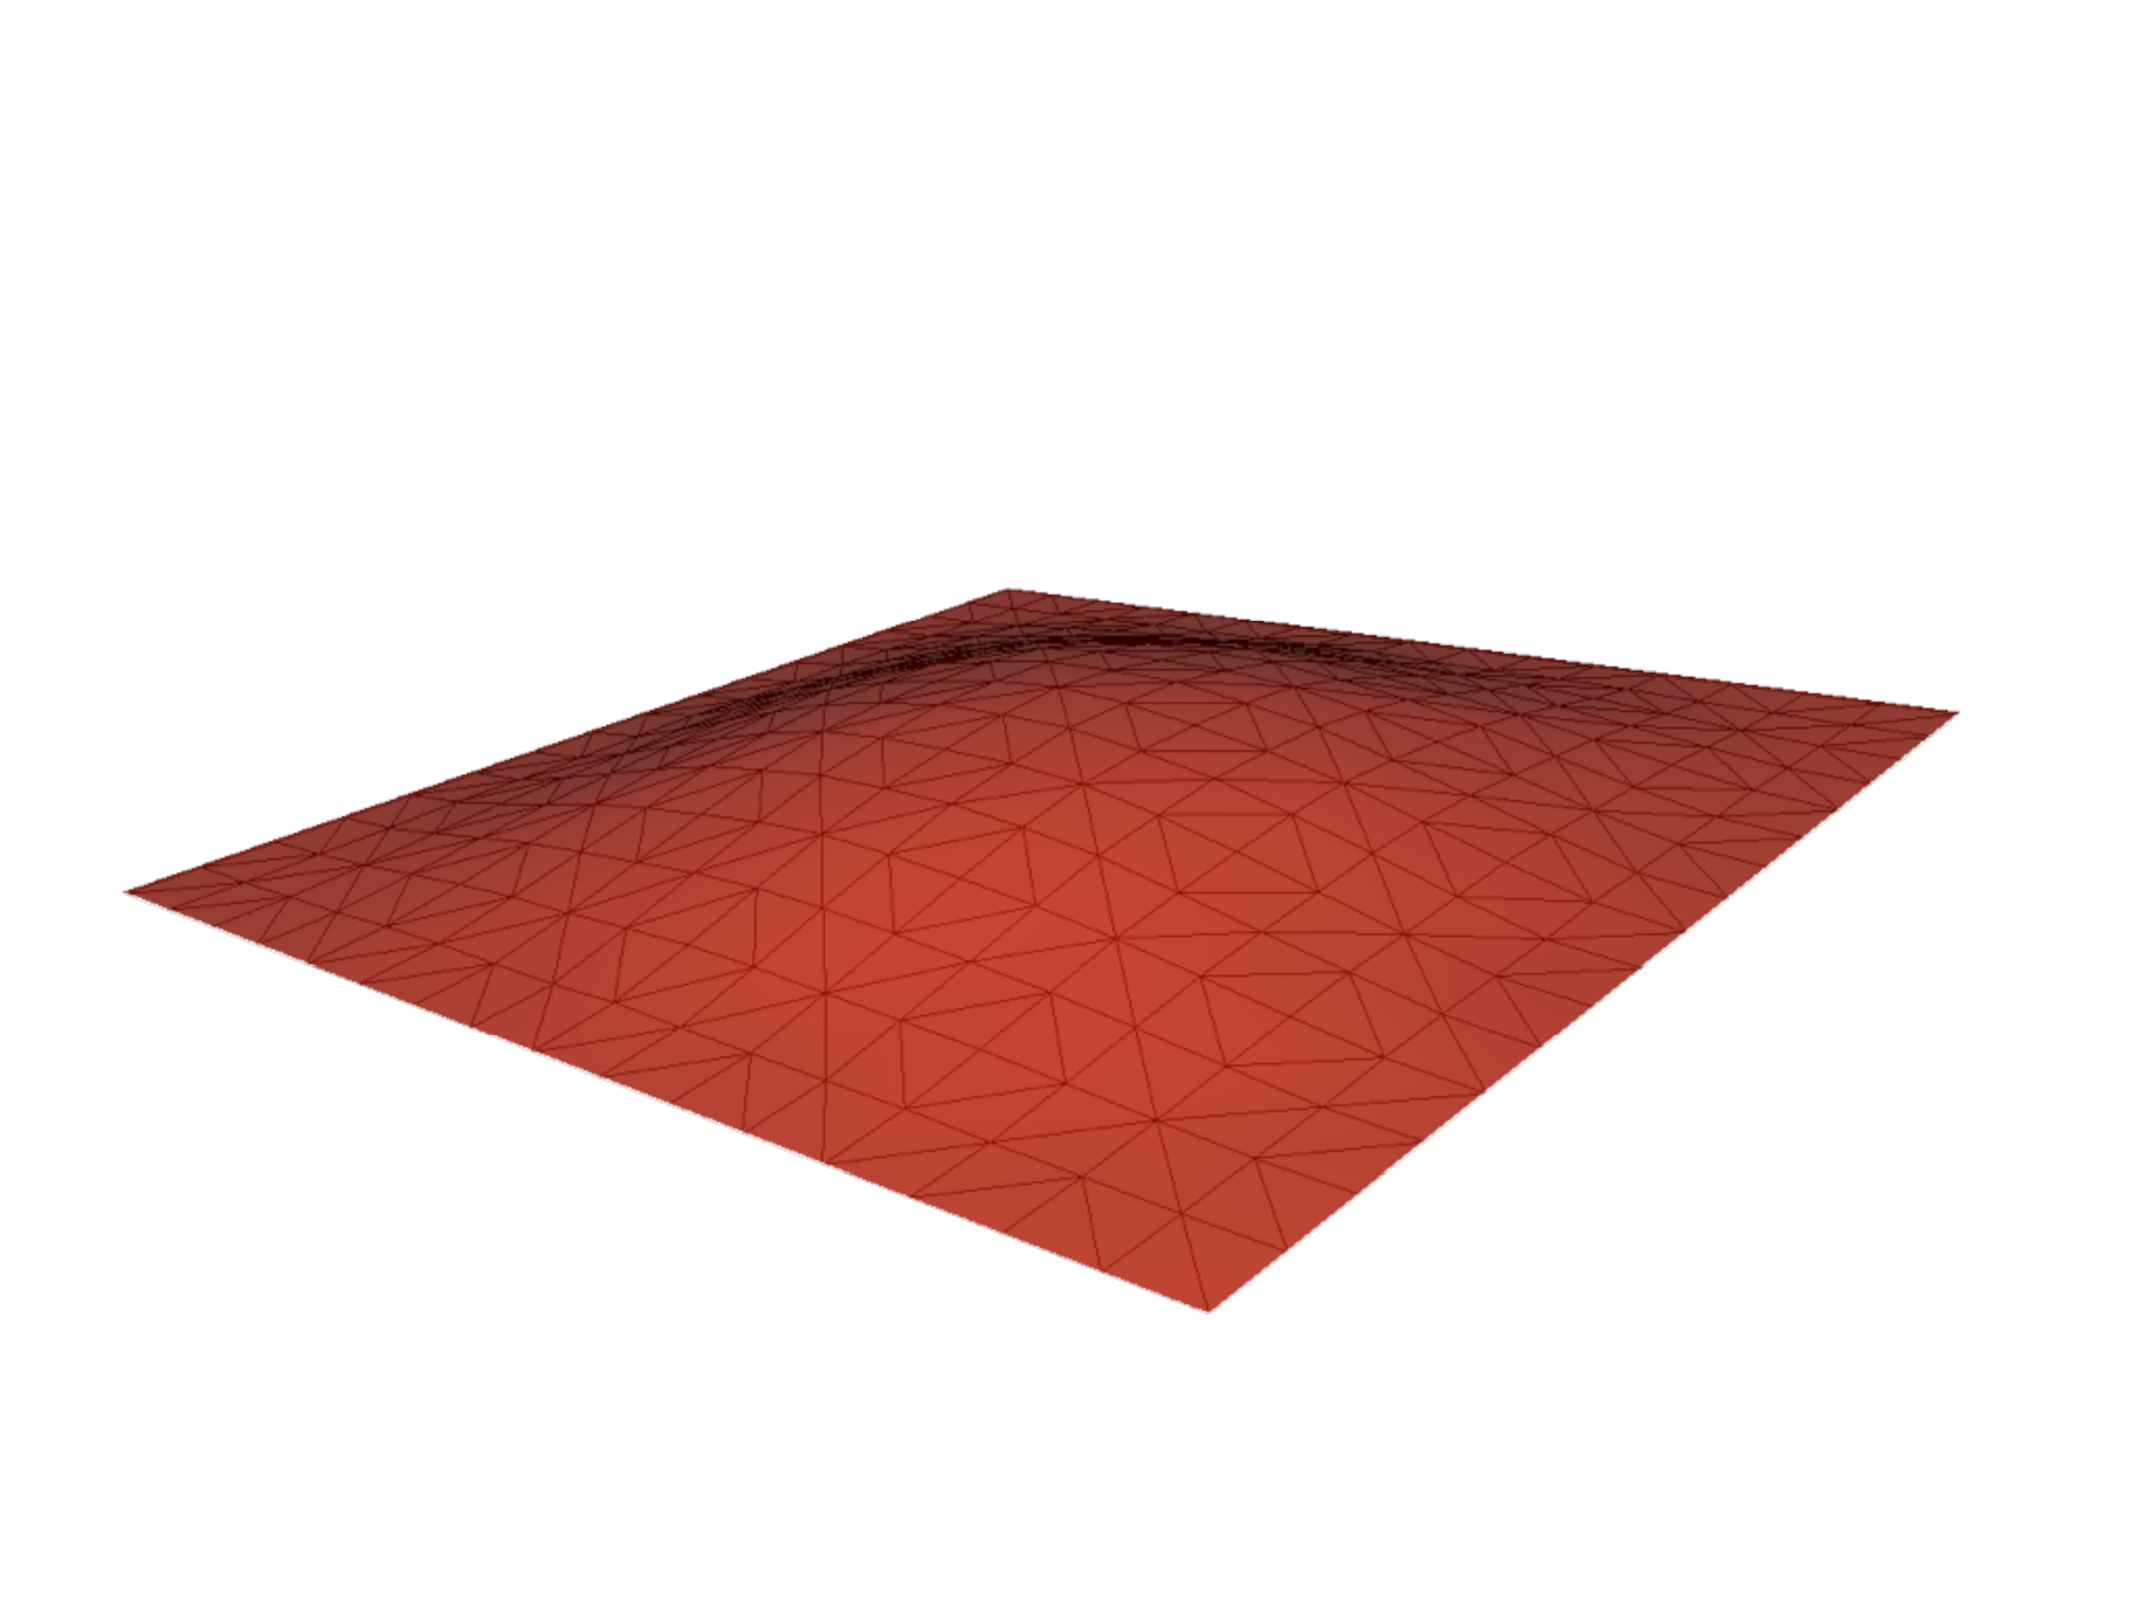
\includegraphics[height=3.5cm]{chapter9/clamped_square.pdf}} & $q$ & $z_{max}$ \tabularnewline
	\cline{2-3}
	& $\,1\,$ & $\, 0.1218 \,$ \tabularnewline
	& $\,2\,$ & $\, 0.2475 \,$ \tabularnewline		
	& $\,3\,$ & $\, 0.3747 \,$ \tabularnewline	
	& $\,4\,$ & $\, 0.5050 \,$ \tabularnewline		
	& $\,5\,$ & $\, 0.6374 \,$ \tabularnewline
	\cline{2-3}
	\end{tabular}
	\vspace{1cm}
	\caption{Comparison of our shell model with theoretical results on the bending of a square plate. An error of less than $1\,\%$ was found between our simulation and theoretical results.}
	\label{chap9:tab-results}
\end{table}


\section{Application to implant deployment simulation in cataract surgery}

Cataract surgery consists in three main steps: capsulorhexis, phacoemulsification, and implantation of an intra-ocular lens. Prior to starting the surgery, a viscoelastic fluid is introduced into the capsule to facilitate capsulorhexis creation and provide protection during phacoemulsification. This fluid remains in the capsule for the duration of the surgery, including the injection of the implant. Capsulorhexis is the technique used to remove a part of the anterior lens capsule. Phacoemulsification consists in using a surgical device which tip vibrates at an ultrasonic frequency to emulsify the natural lens material and then aspirate the fragments of the cortical material. After the removal of the diseased lens, an intra-ocular lens is implanted into the eye, through a small incision (about $2\,$mm) using a foldable intra-ocular lens (see \fig{chap9:fig-surgery}). The foldable lens, usually made of acrylic material, is then implanted within the lens capsule through the incision used during phacoemulsification. In some cases the implant can be flipped or  the hooks (also called \emph{haptics}) can break. Therefore the simulation of the insertion and deployment of the implant is crucial for achieving a successful surgery.
%
\begin{figure}[ht]
\centering 
\subfloat[ ]{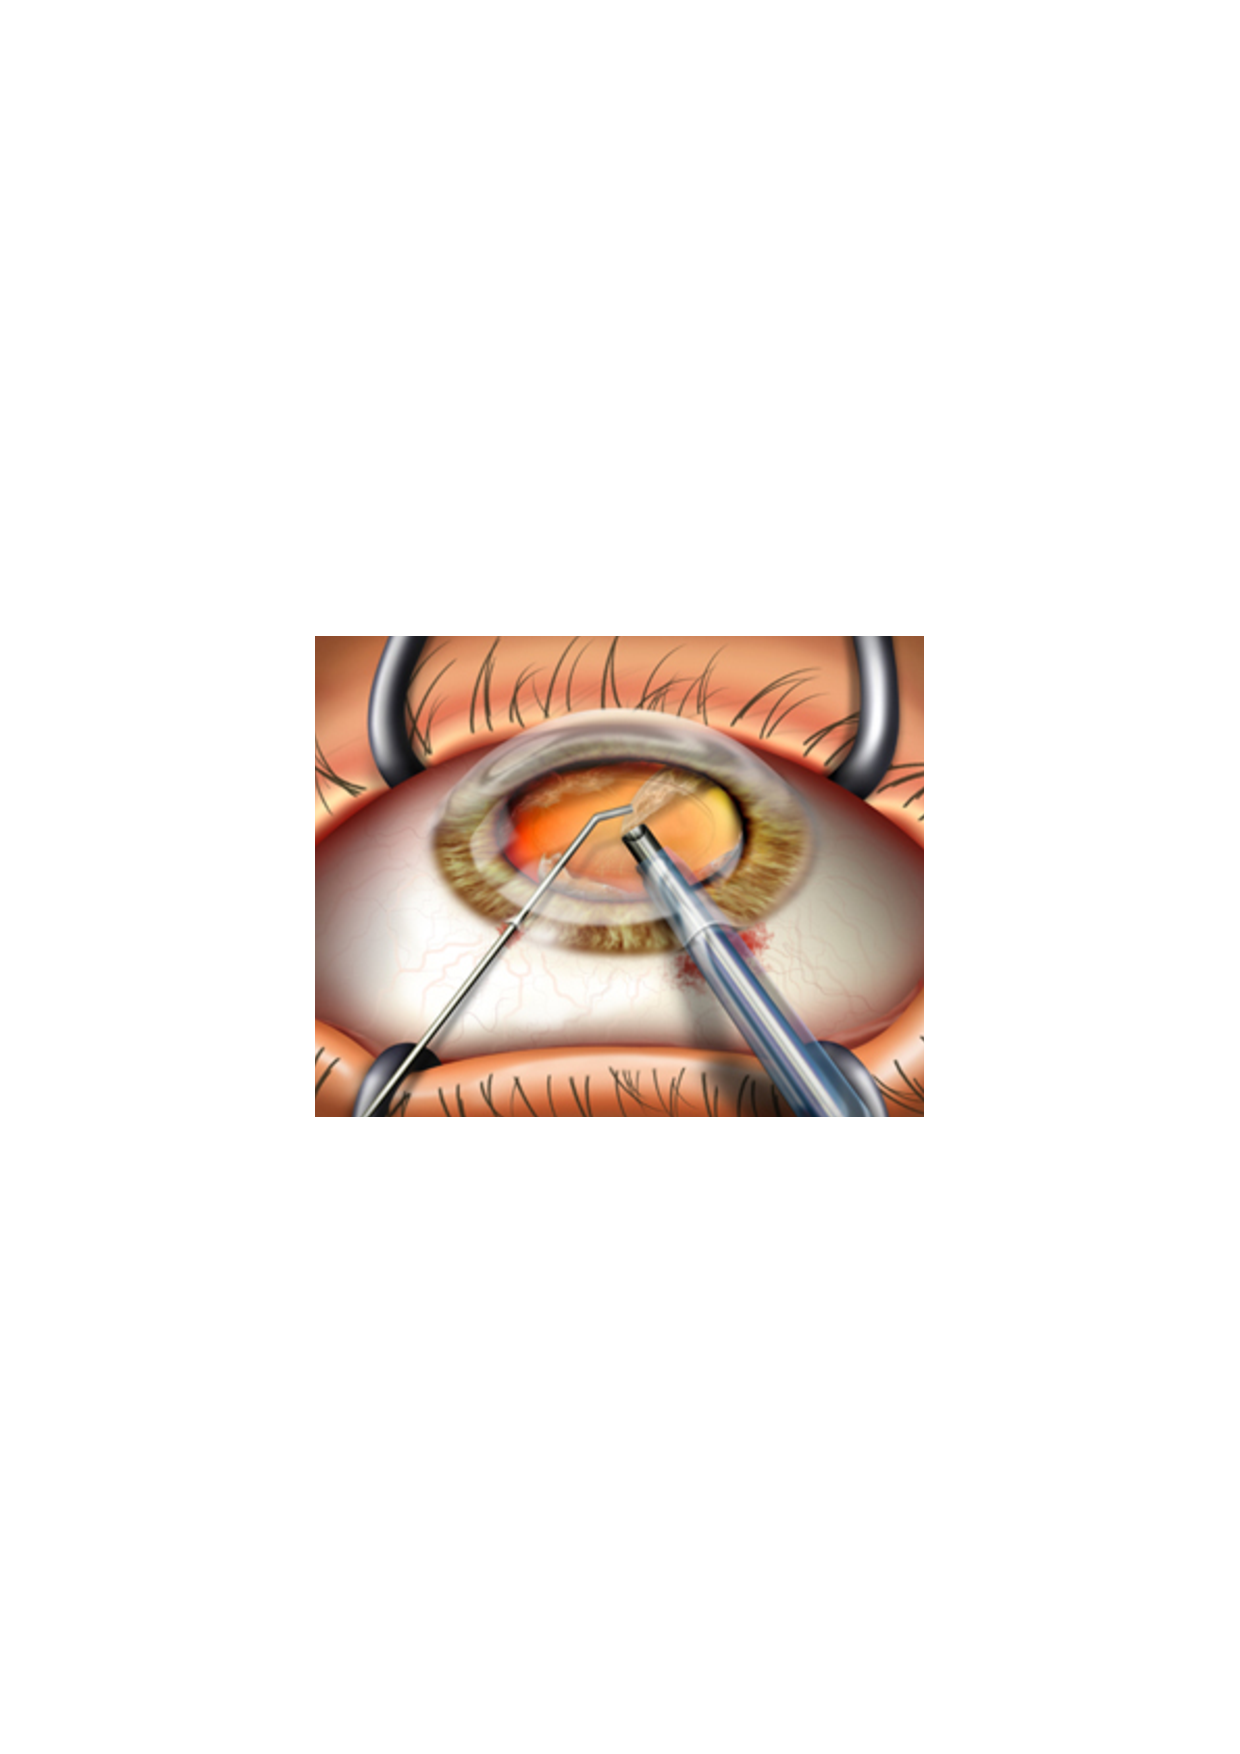
\includegraphics[height=3.2cm]{chapter9/suction.pdf}}
\hspace{1cm} 
\subfloat[ ]{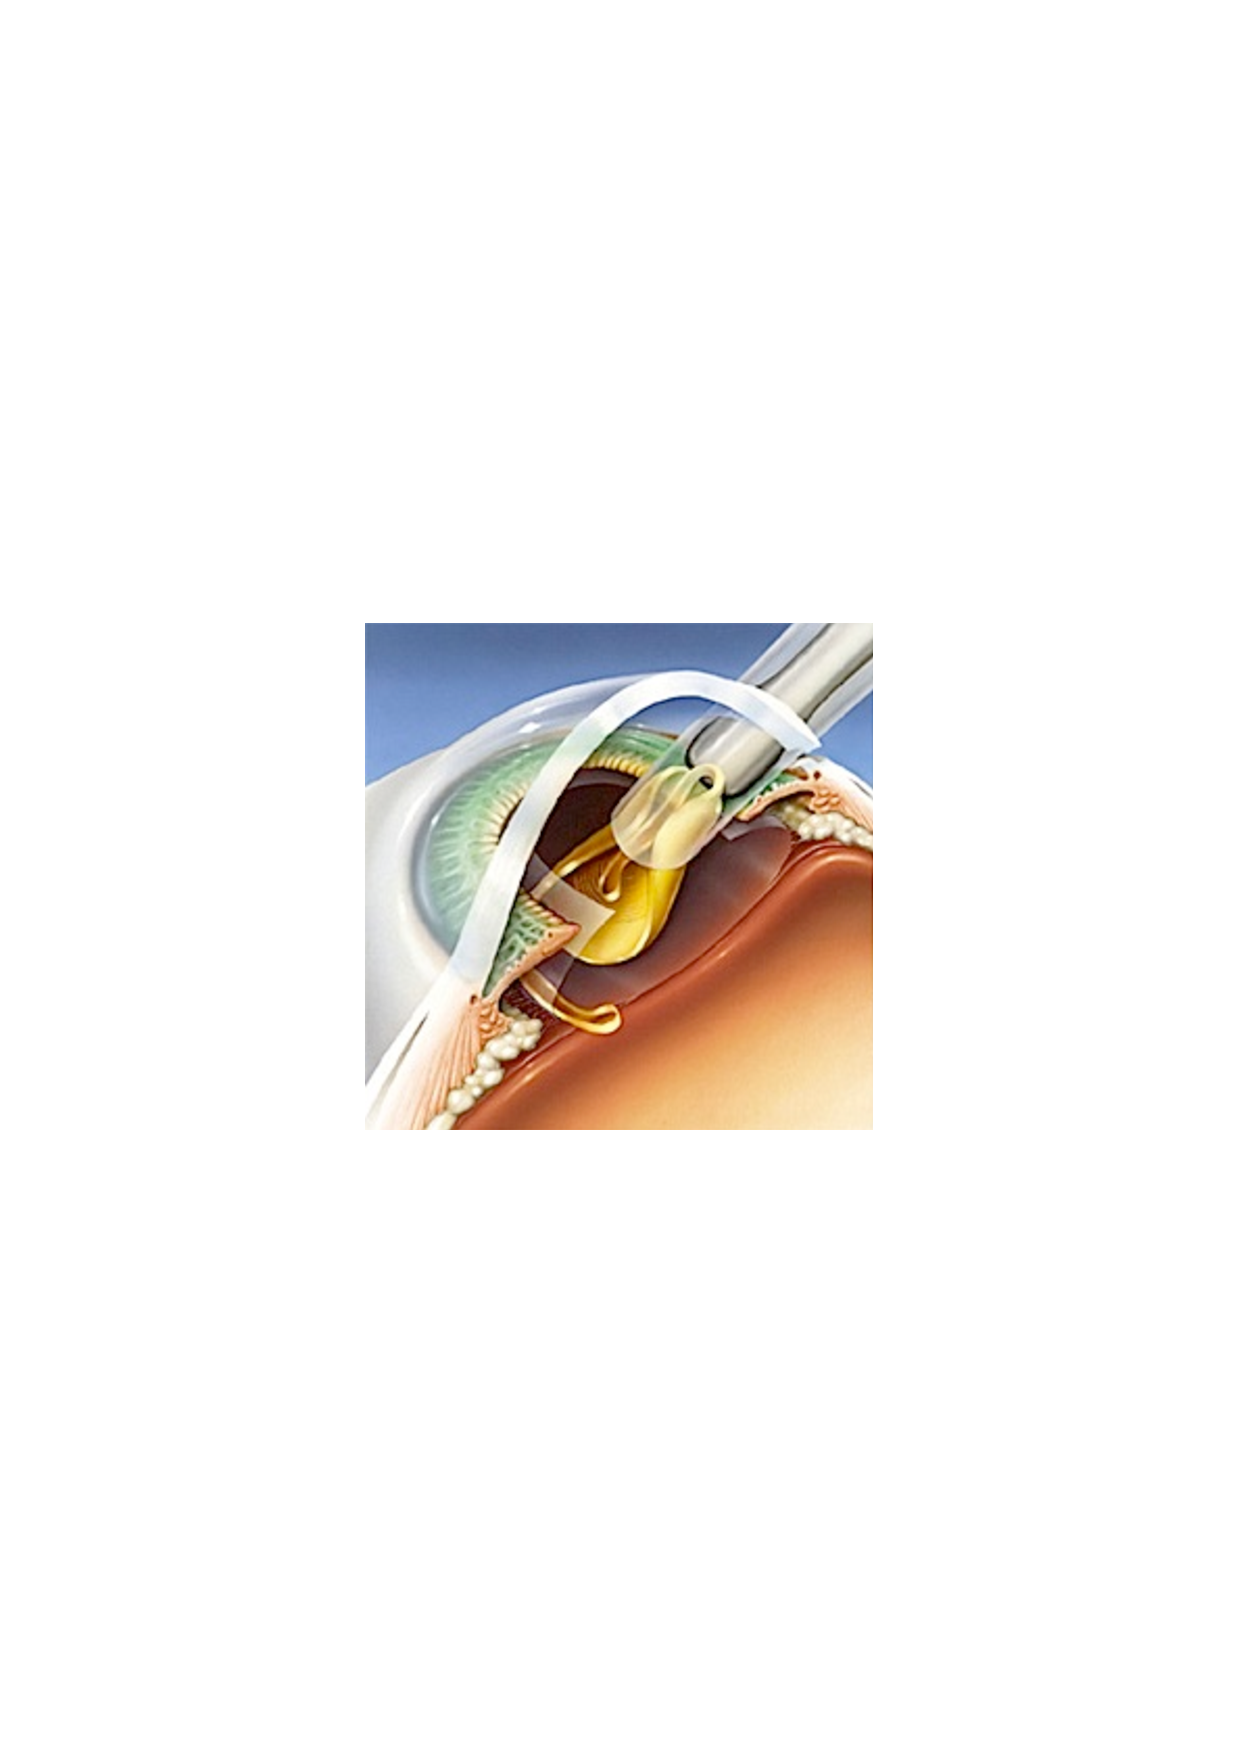
\includegraphics[height=3.2cm]{chapter9/implant_injection_step_1.pdf}}
\hspace{1cm} 
\subfloat[ ]{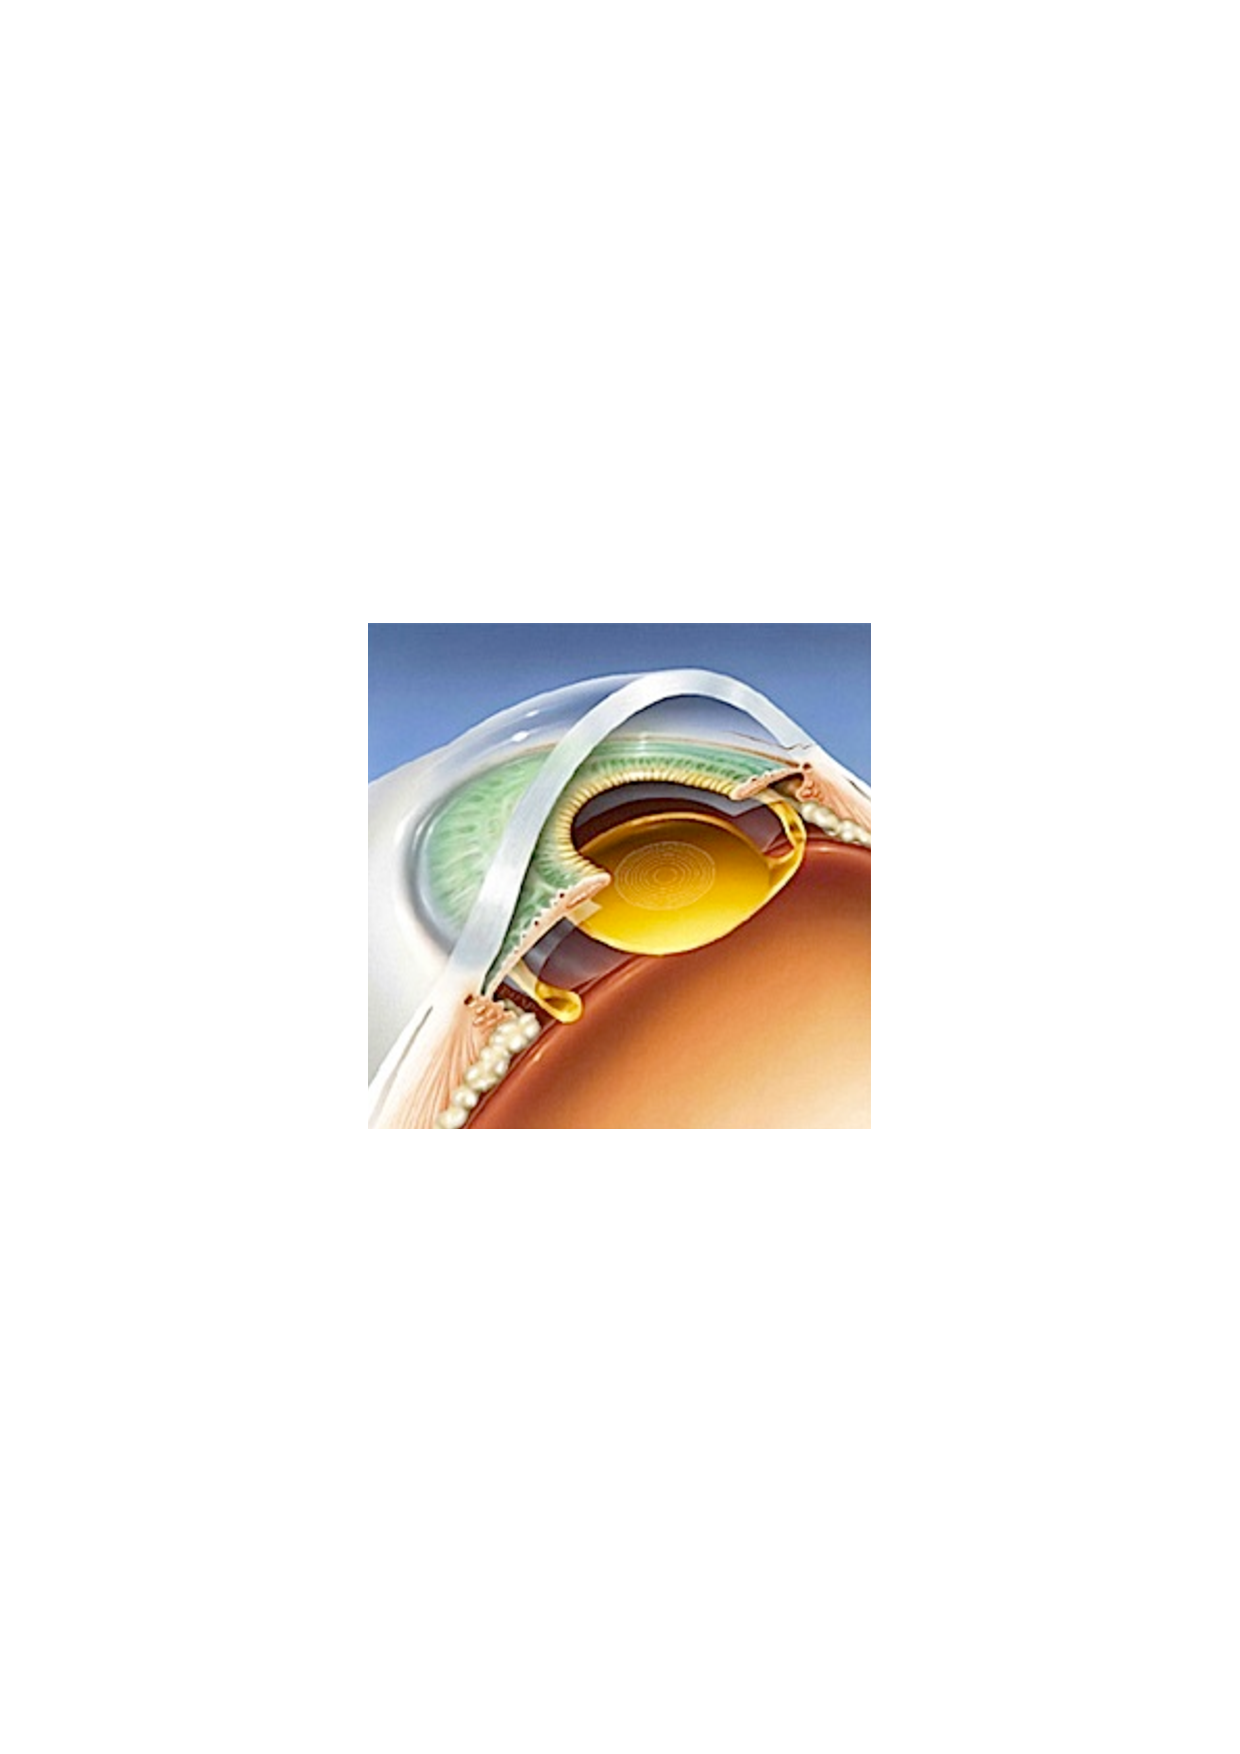
\includegraphics[height=3.2cm]{chapter9/implant_injection_step_2.pdf}}
\caption [Steps of cataract surgery] {(a) removal of the opacified lens by phacoemulsification. (b) insertion of the lens implant which is folded inside the injection device and then deploys within the lens capsule. (c) the lens in place in the capsule.}
\label{chap9:fig-surgery}
\end{figure}

To simulate the insertion and deployment of an intra-ocular lens, we first created a triangulation of the lens surface. Particular care was given to the mesh, to ensure that areas where large stresses occur contain a higher density of elements (see \fig{chap9:fig-mesh}). This was done by noting the constraints applied by the surgeon to the haptics while inserting the implant within the injection device. During this stage, the haptics are folded onto the implant body, leading to high stresses at the junctions. The lens mesh contains $743$ triangles and $473$ nodes. Models of the injection device and the entire eye anatomy were also created. Physical parameters of the lens implant have been provided by the manufacturer Alcon and they are presented in Table~\ref{chap9:tab-parameters}.
%
\begin{table}[ht]
	\begin{center}
		\begin{tabular}{|p{3cm}|p{3cm}|p{3cm}|}
		\hline
		 \centering Young's modulus & \centering Poisson's ratio & \centering Mass density \tabularnewline
		\hline
		\centering $1\,$MPa & \centering $0.42$ & \centering $1.2\,$g/cm$^3$ \tabularnewline
		\hline
		\end{tabular}
	\vspace{0.3cm}
	\caption{Physical parameters of the intra-ocular implant (source: Alcon)}
	\label{chap9:tab-parameters}
	\end{center}
\end{table}

The first difficulty is to obtain the folded geometry of the lens within the injection device. This step is not important for the training process and does not need to be interactive. Indeed the surgeon does not always have to prepare the implant as some injection devices are readily available with a folded implant already in place. We simulate the folding process by first folding the haptics onto the implant body. The body was then bent while keeping the haptics inside to obtain the shape described in \fig{chap9:fig-implantFolding}. The whole process was carried out by applying the necessary forces and boundary conditions on the body and haptics of the implant. The folded implant was then placed into the injection device. The simulation of the injection consists in pushing the intra-ocular implant within the injection device into the lens capsule. During these stages of the simulation, complex contacts occur and consist of self collisions of the lens as well as collisions between the lens and the injector and later with the capsule. To solve the contacts we use the contact warping method proposed by \cite{Saupin08} as it offers an efficient way to compute physically correct contact responses in the case of co-rotational models \TODO{is it still true? I'm not even sure we used this technique in the final submission to ISBMS}. As adhesions between the haptics and the body is often observed in surgery, friction is also taken into account in the contact response process.
%
\begin{figure}[ht]
\centering 
\subfloat[Real implant]{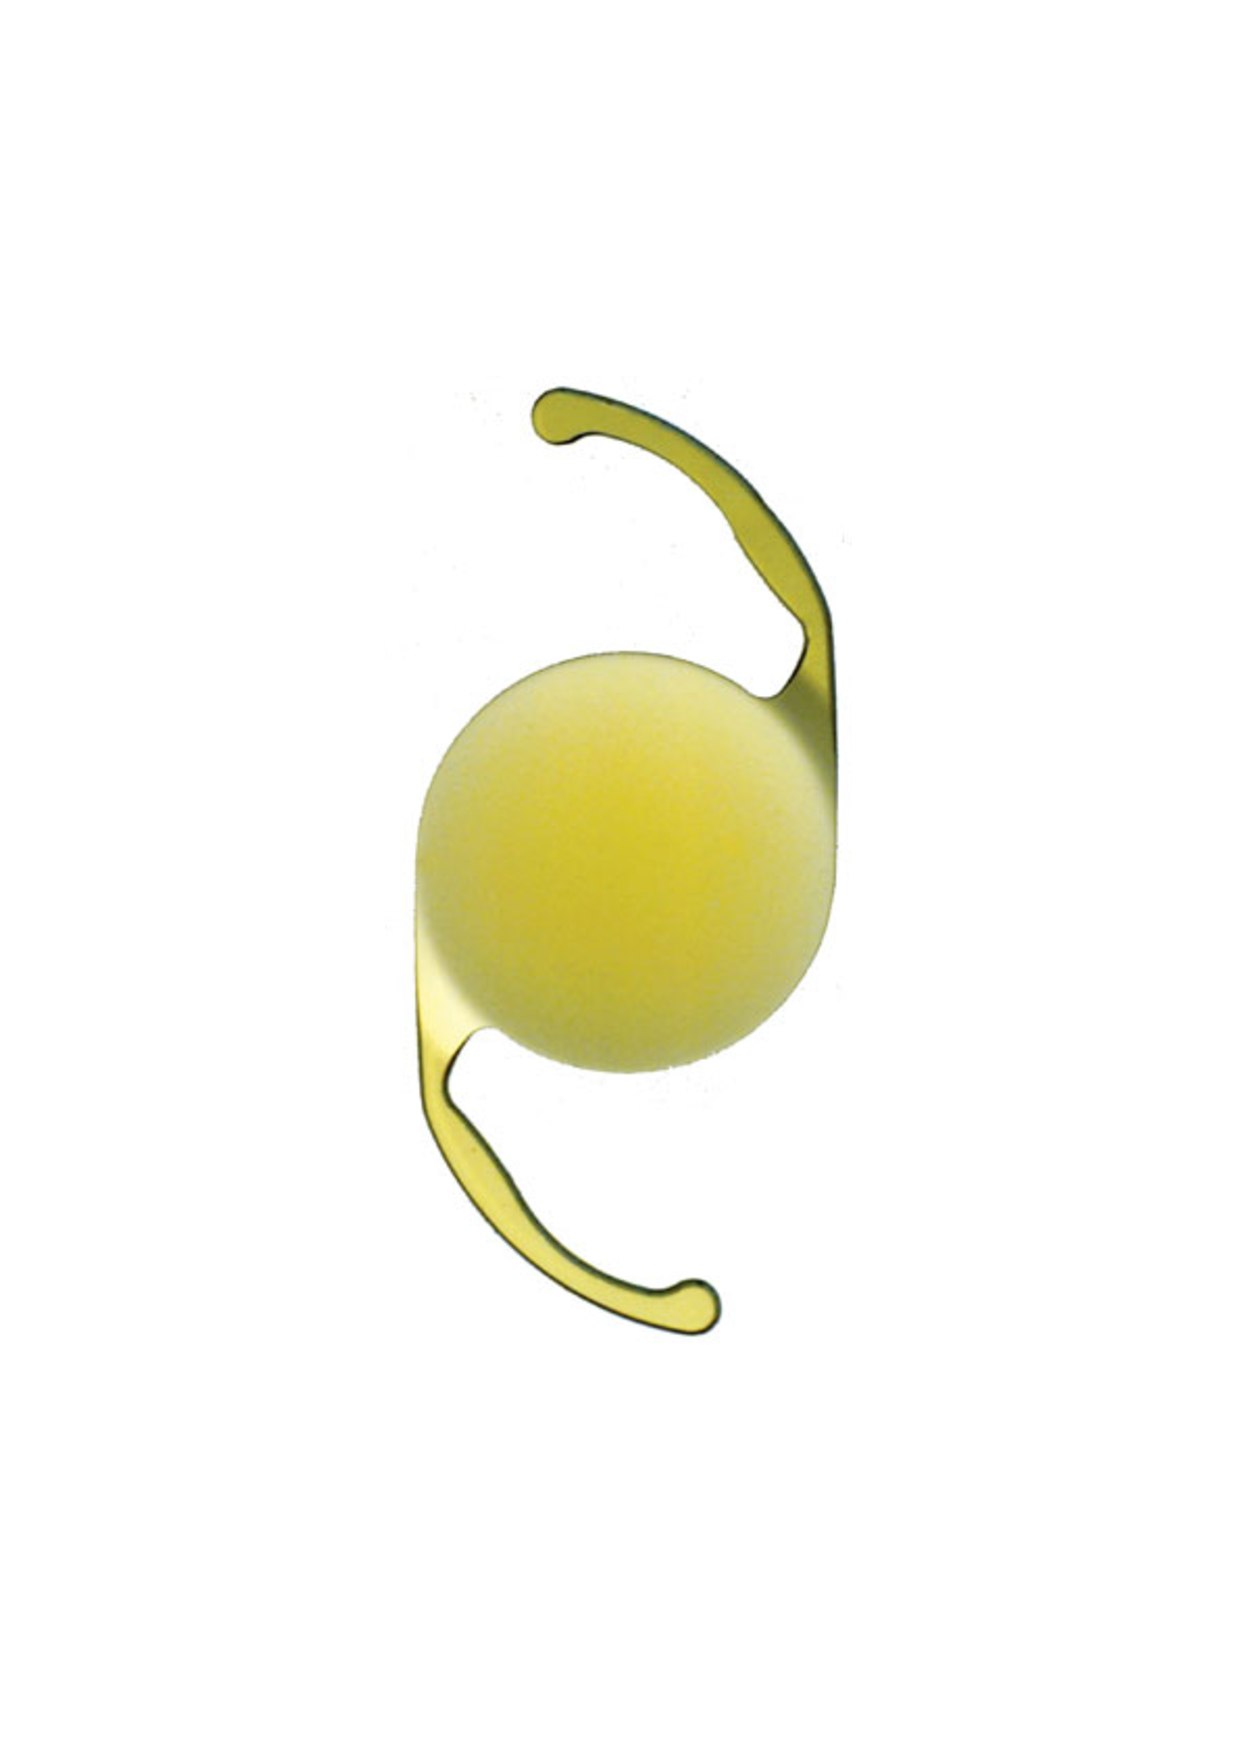
\includegraphics[height=5cm]{chapter9/IOL.pdf}}
\hspace{1cm} 
\subfloat[Meshed model]{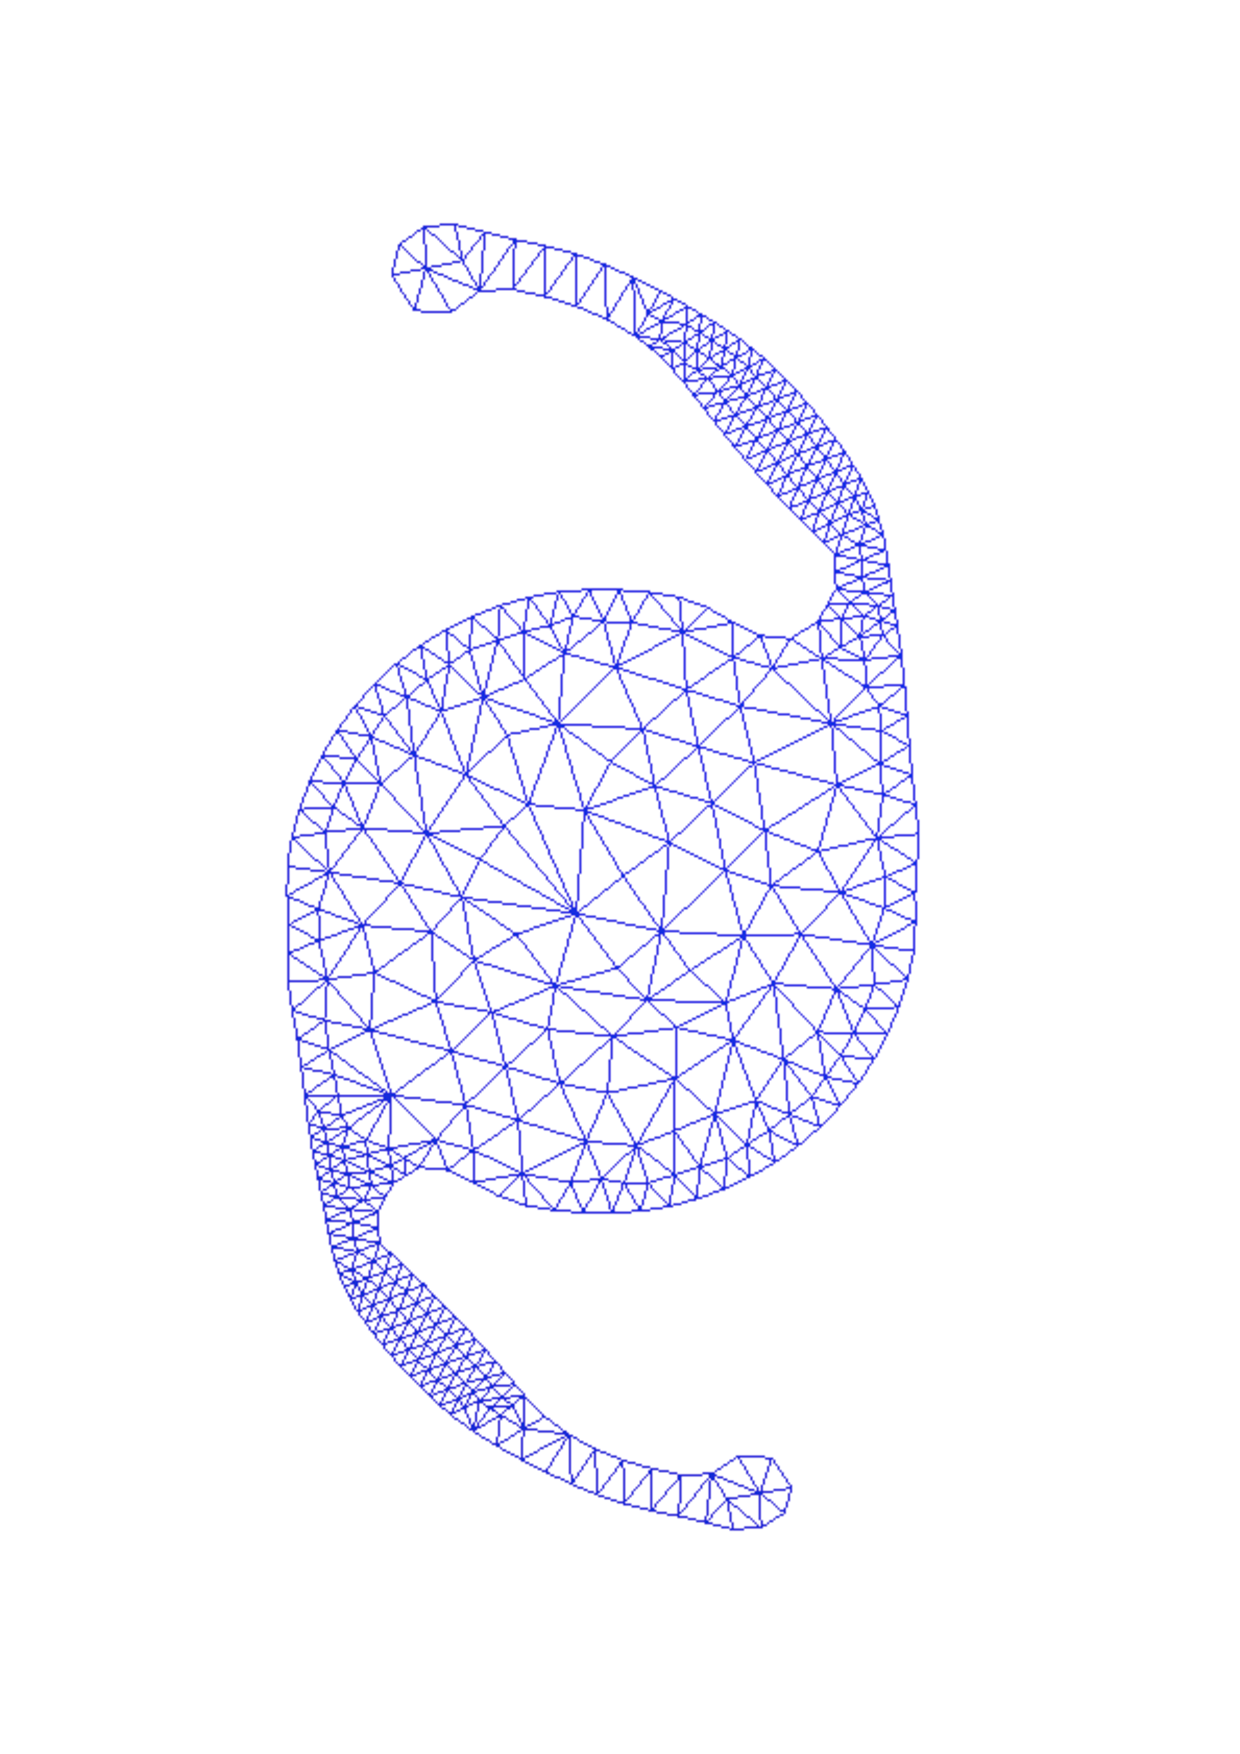
\includegraphics[height=5cm]{chapter9/mesh_implant.pdf}}
\caption [Lens implant and its mesh] {An actual intra-ocular implant (a) and the triangular (b) mesh used in our simulations. Notice the higher density of elements in areas where large deformations will take place. Image of implant courtesy of Alcon.}
\label{chap9:fig-mesh}
\end{figure}

\begin{figure}[ht]
\centering
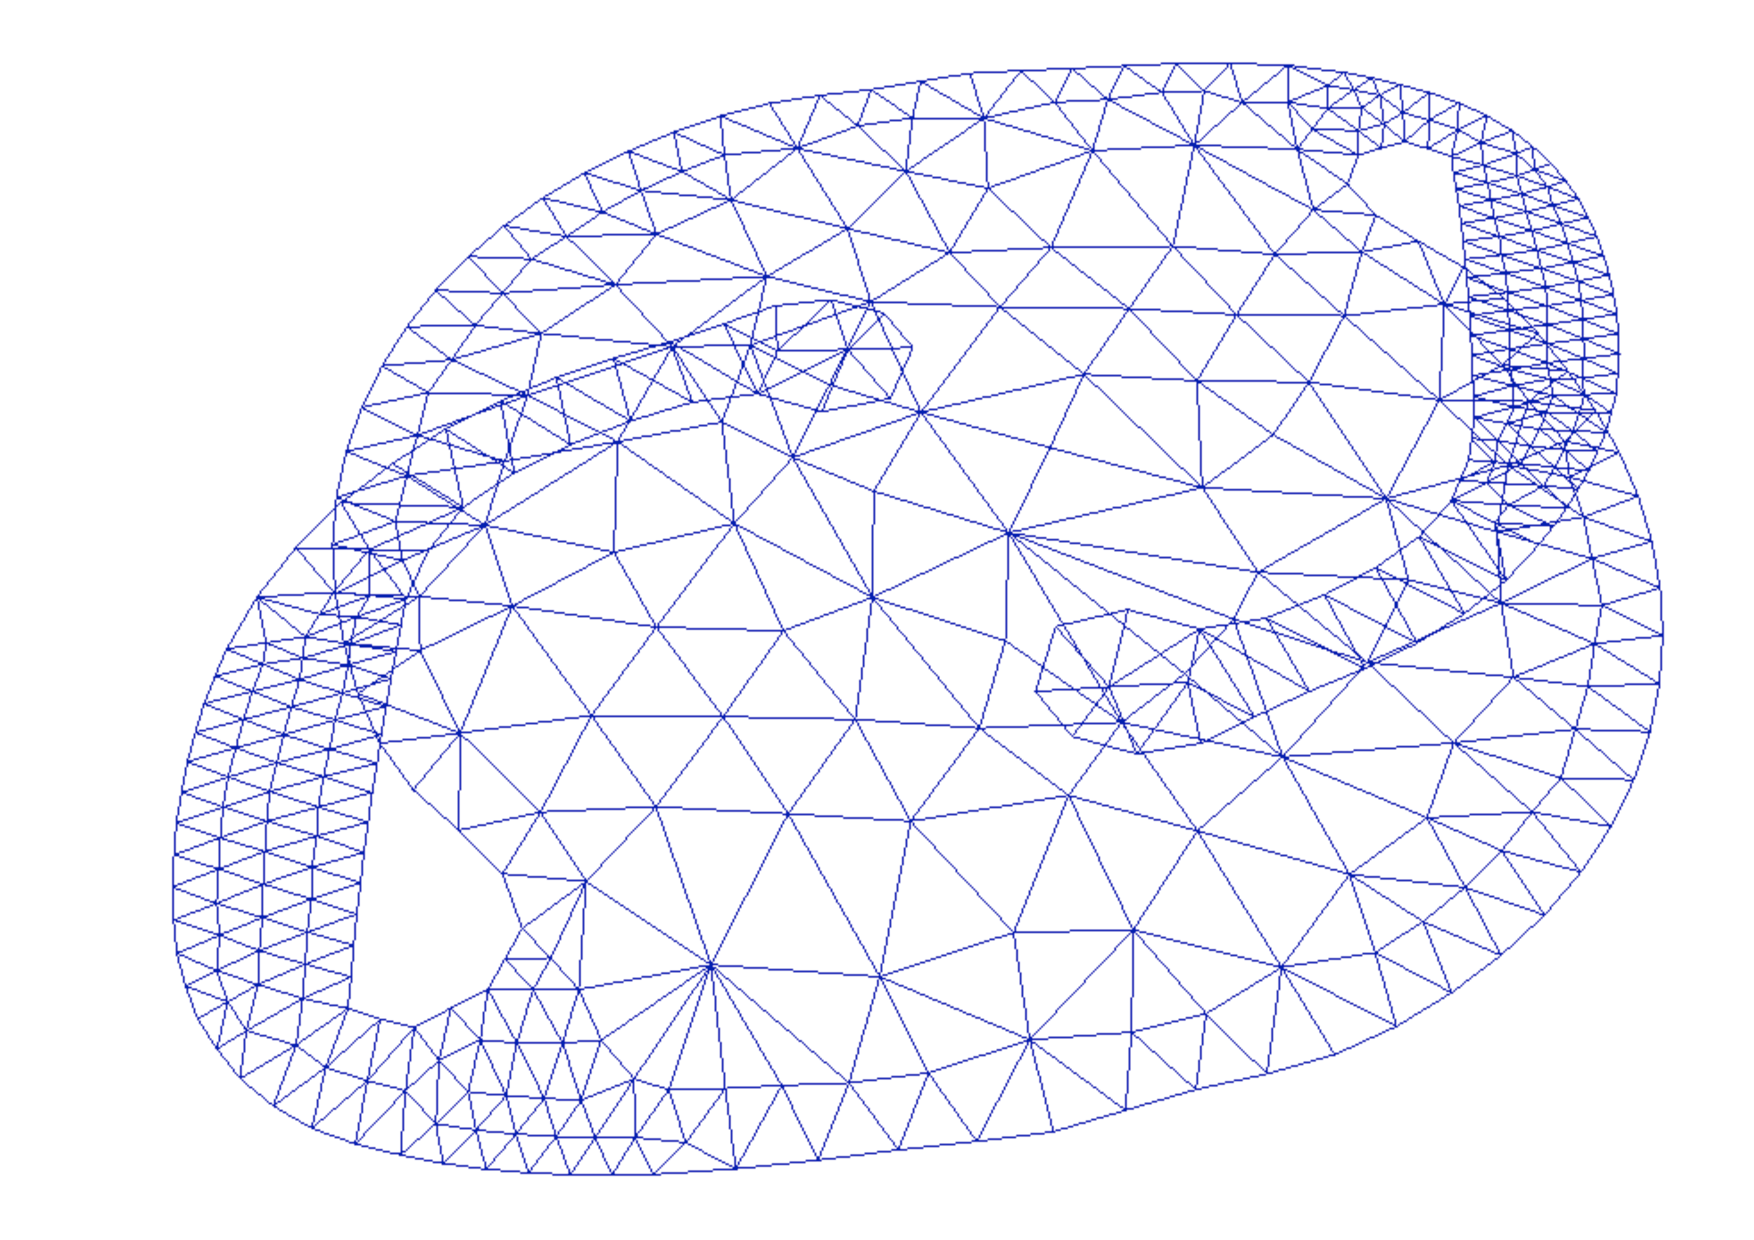
\includegraphics[width=5cm]{chapter9/implant_folding1.pdf}
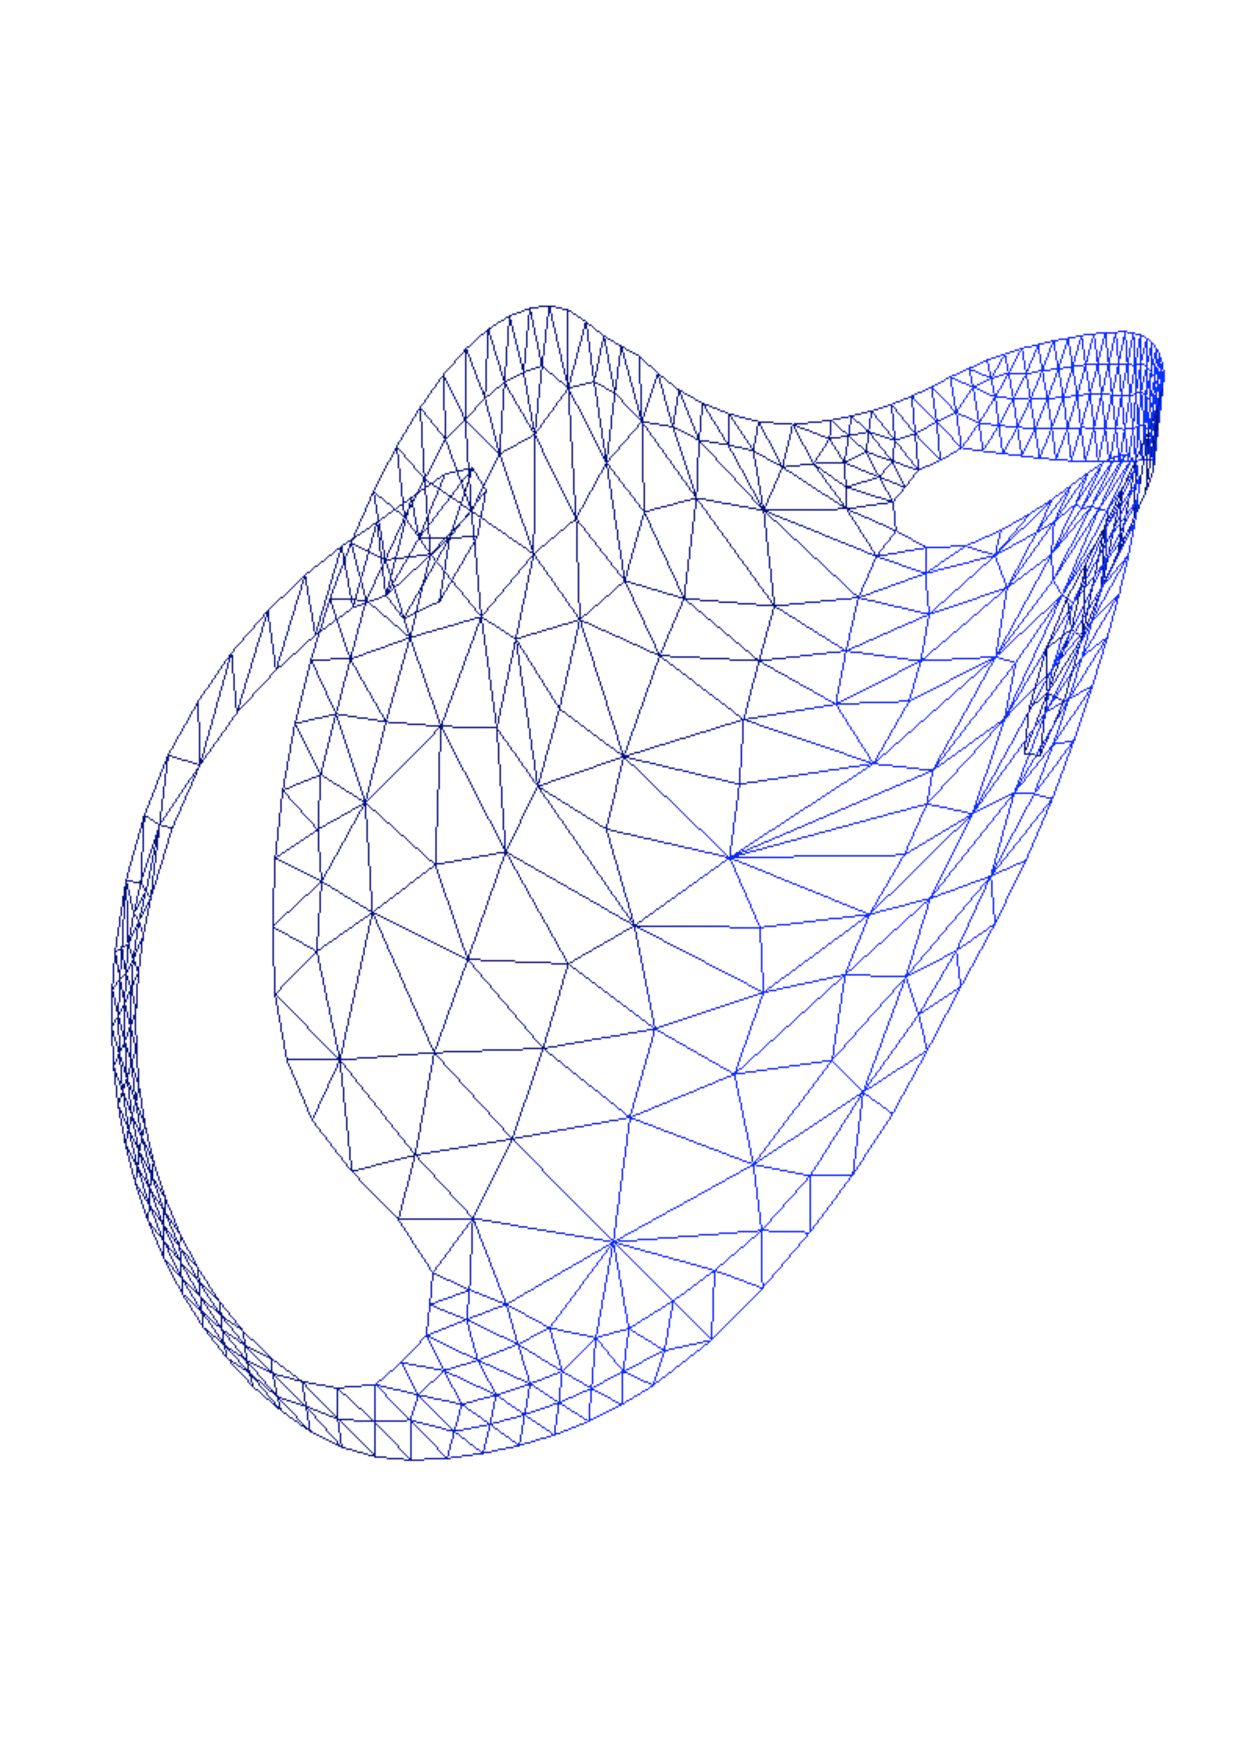
\includegraphics[width=4.5cm]{chapter9/implant_folding2.pdf} \\
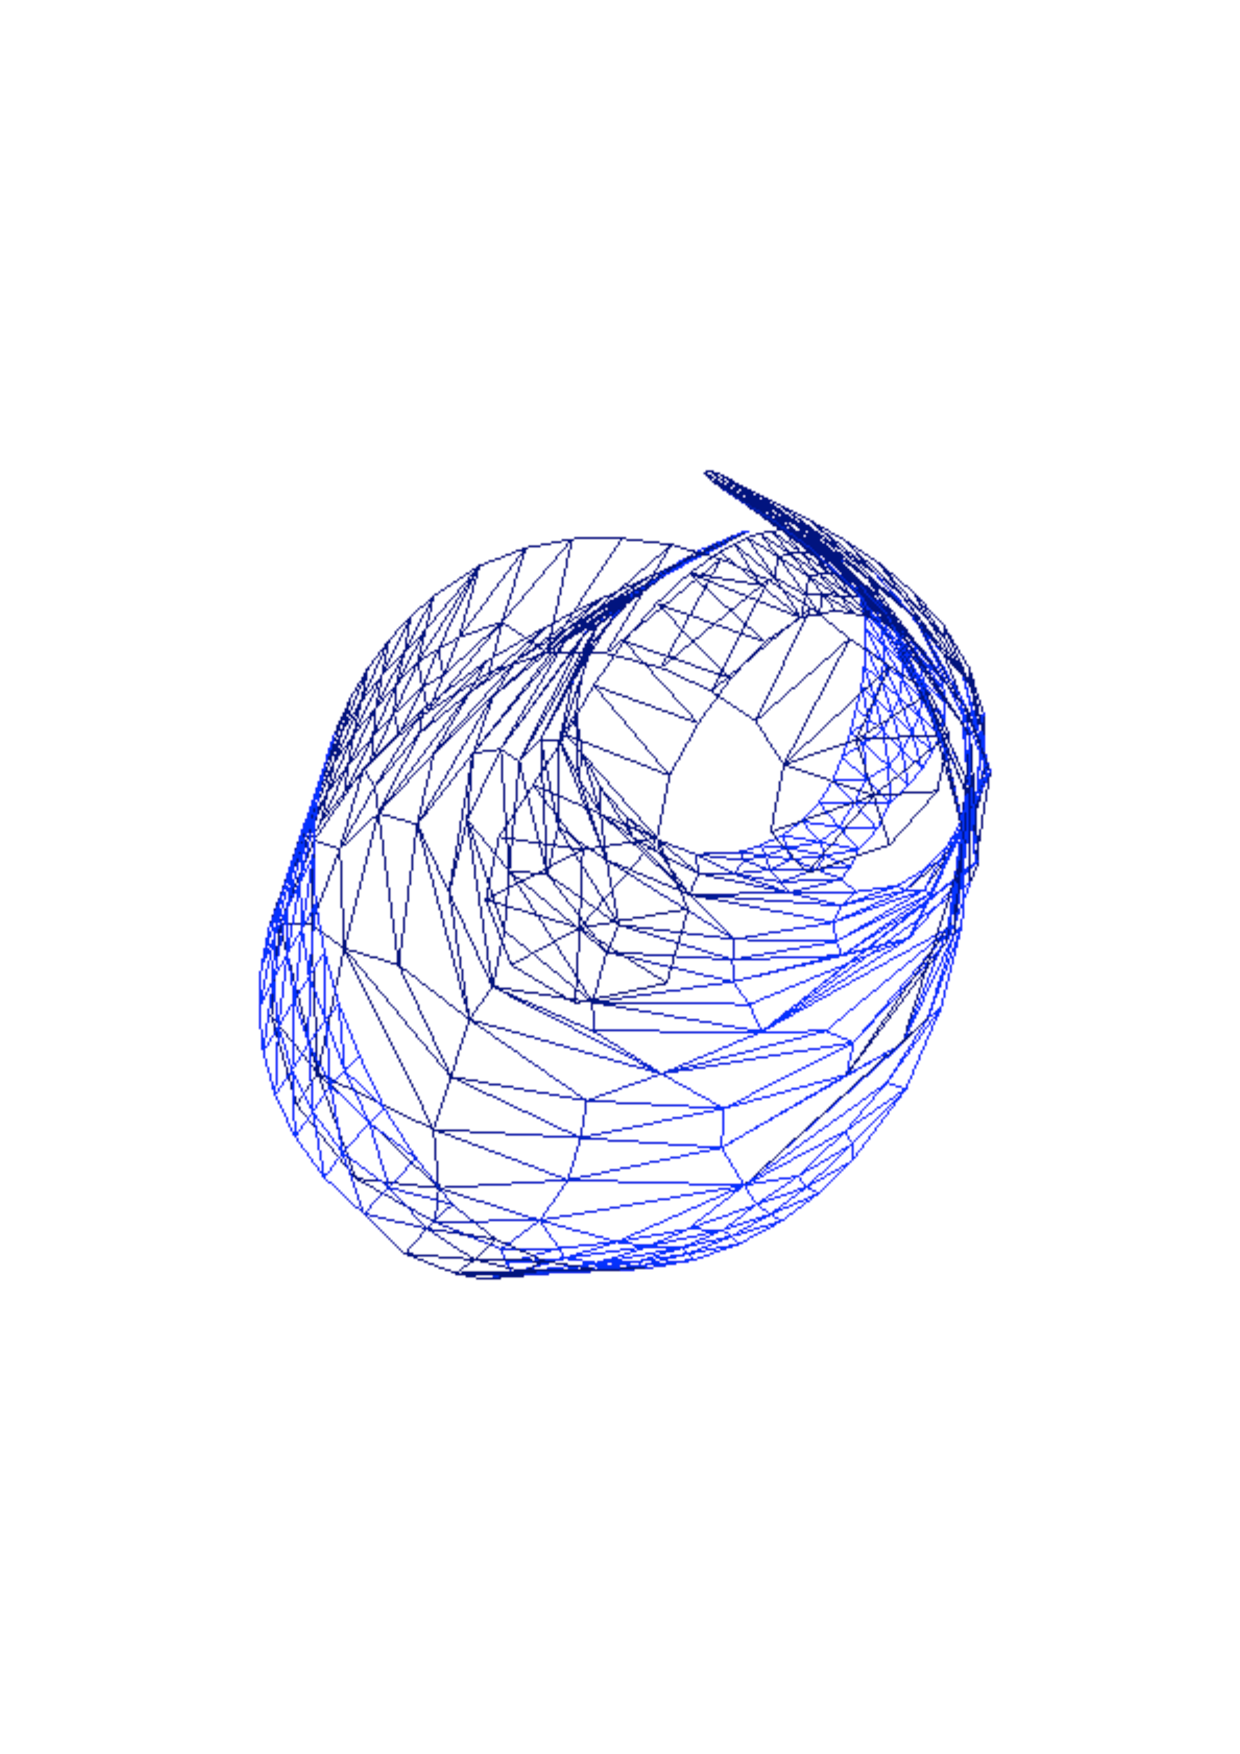
\includegraphics[width=4cm]{chapter9/implant_folding3.pdf}
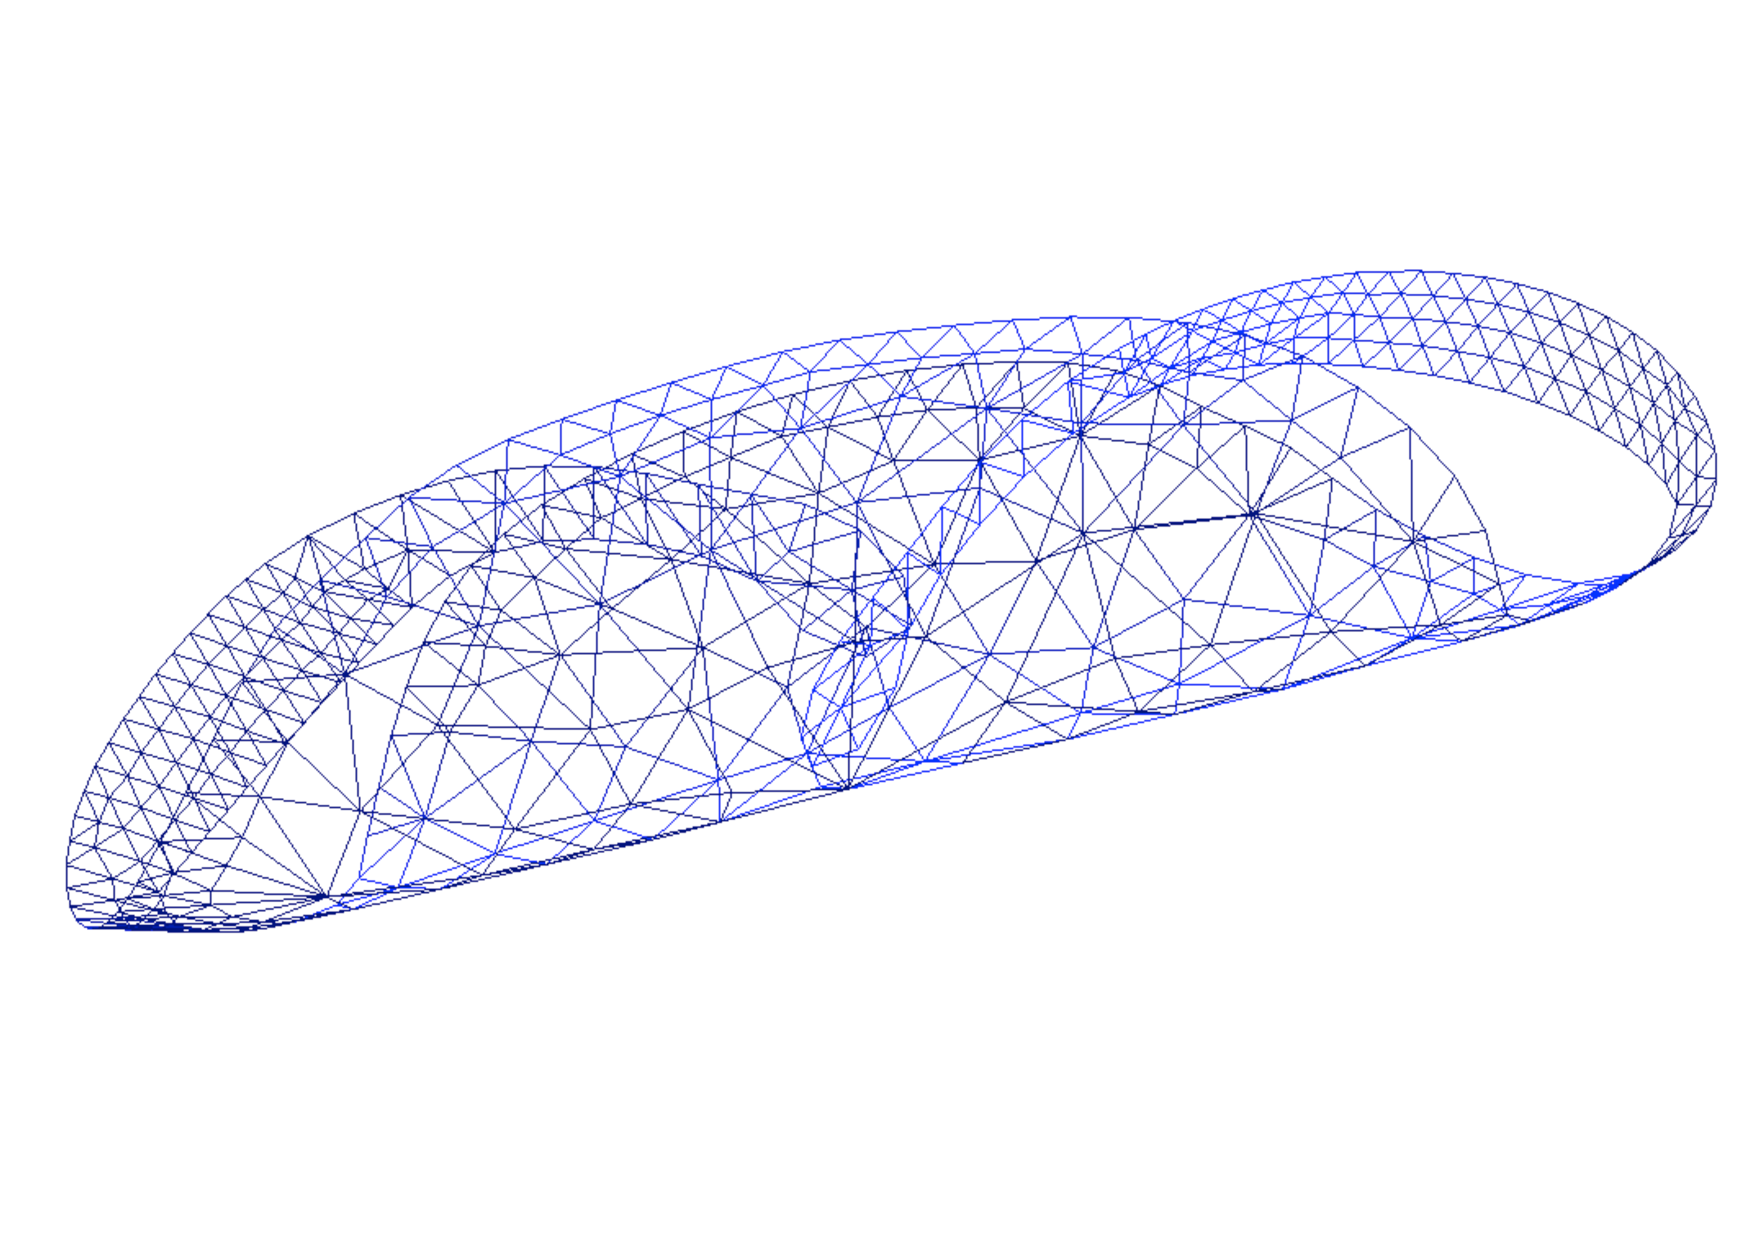
\includegraphics[width=7cm]{chapter9/implant_folding4.pdf}
\caption [Folding of intra-ocular implant] {Top: intermediary steps of the intra-ocular implant folding. Bottom: fully folded implant ready to be placed into the injection device.}
\label{chap9:fig-implantFolding}
\end{figure}

Results of our simulation are illustrated in \fig{chap9:fig-simu-results}. We can notice the progressive deployment of the implant when it exits the injector.  The shape of the intra-ocular lens remains very close to that of a real one during all stages of the simulation: within the injector, during the ejection phase, and when in place within the capsule. Due to the high stiffness and low mass of the lens, a direct sparse solver was used at each time step (dt $= 0.01\,$s) rather than an iterative solver, resulting in a more accurate and more stable simulation, to the detriment of computation times (about 5 FPS for the complete simulation, and about 10 FPS for the deformation only, on a 2.4 GHz processor).

% Link where images from surgery have been found: http://asianophthalmology.org/articles/?a=articles&p=6
\begin{figure}[ht]
\centering
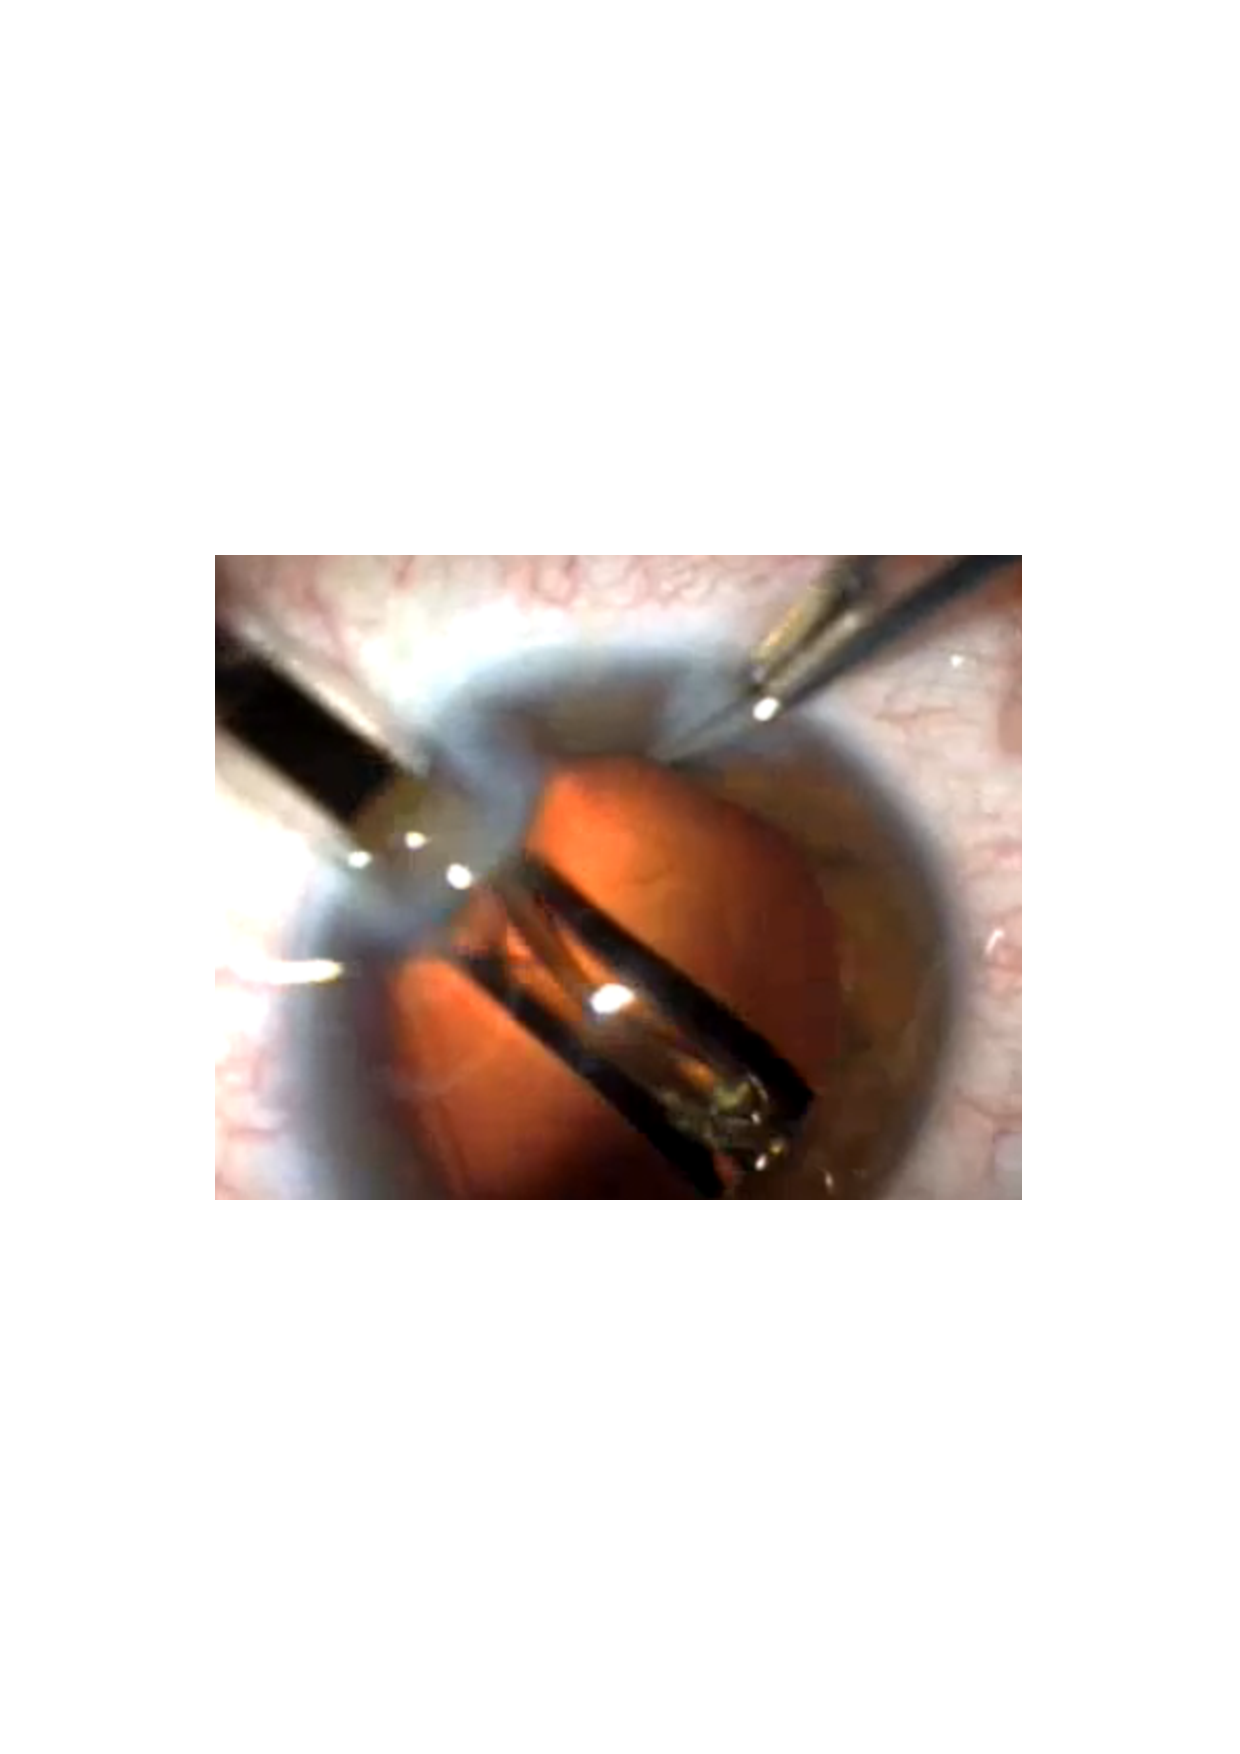
\includegraphics[width=4.5cm]{chapter9/surgery1.pdf}
\hfill
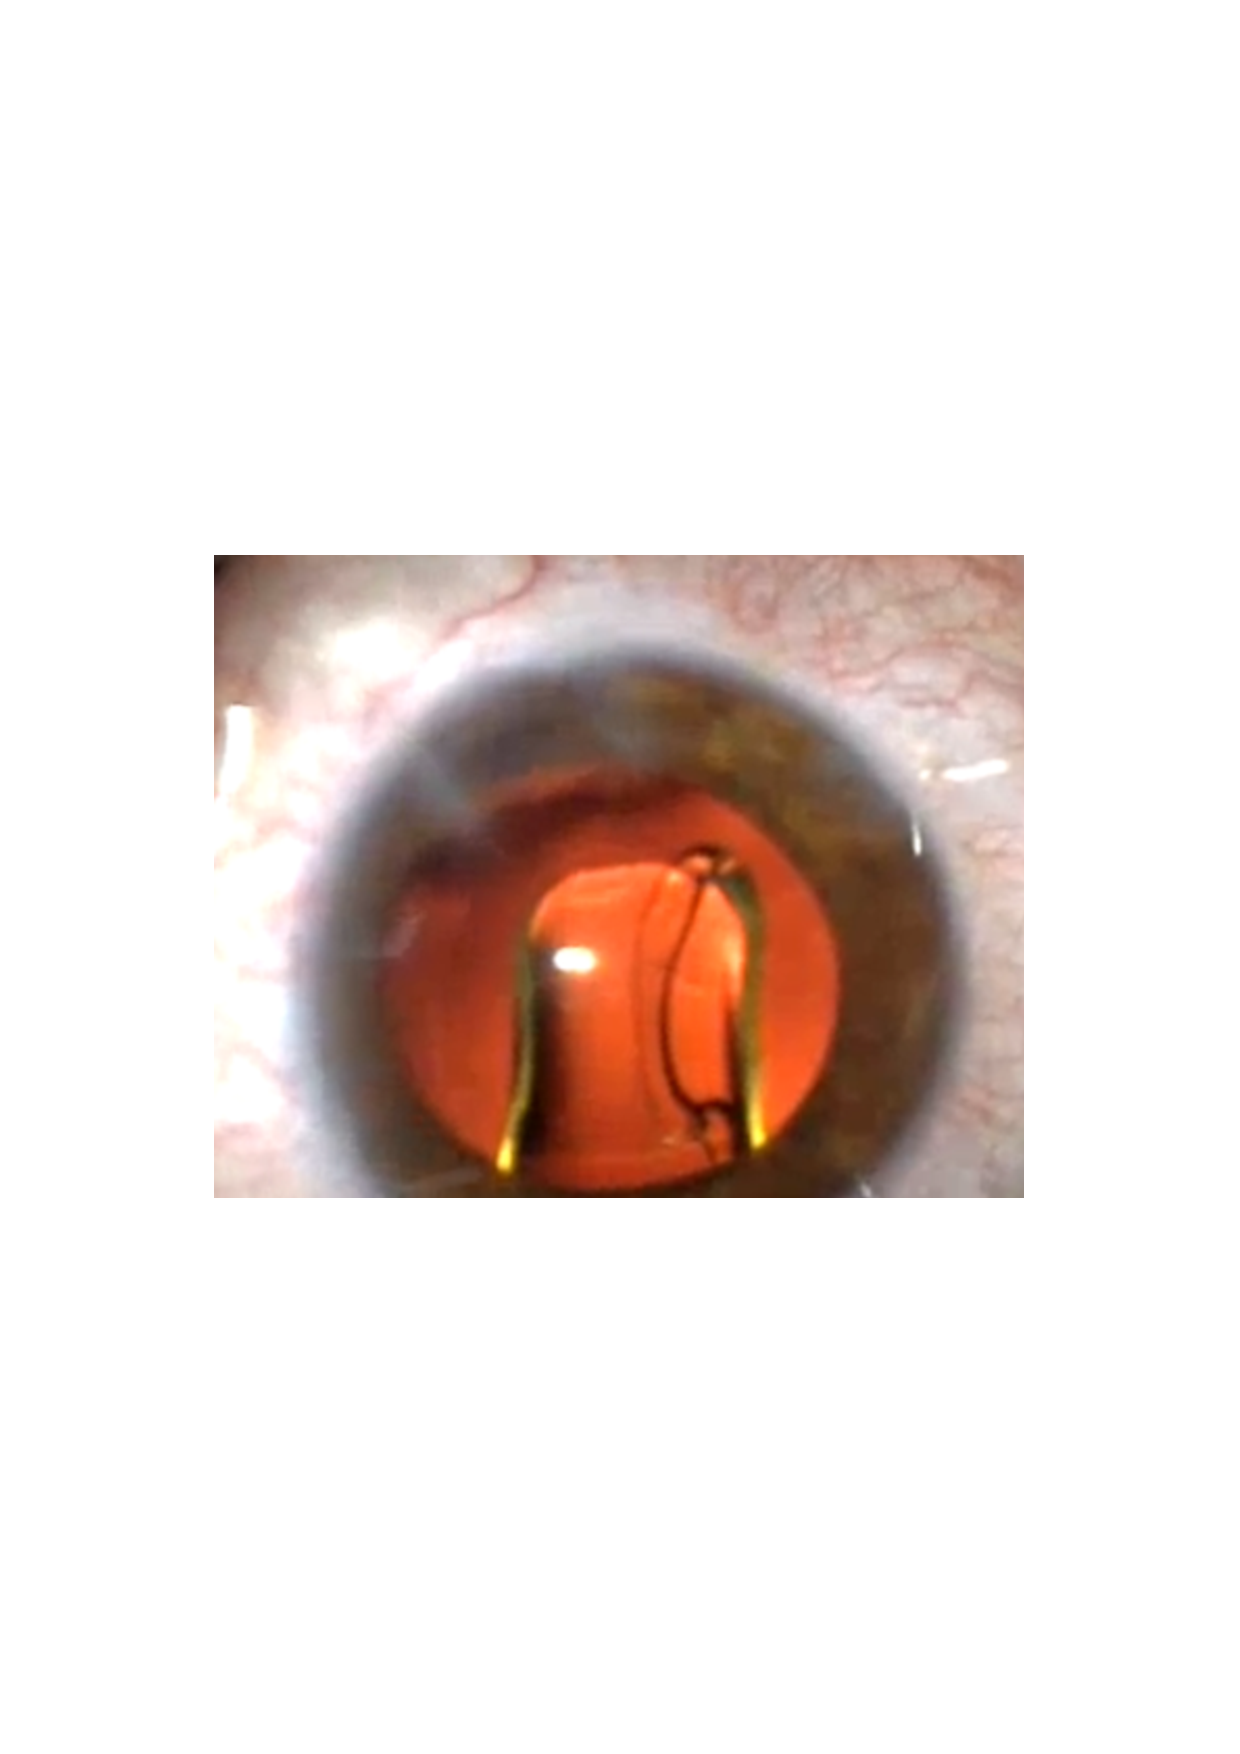
\includegraphics[width=4.5cm]{chapter9/surgery2.pdf}
\hfill
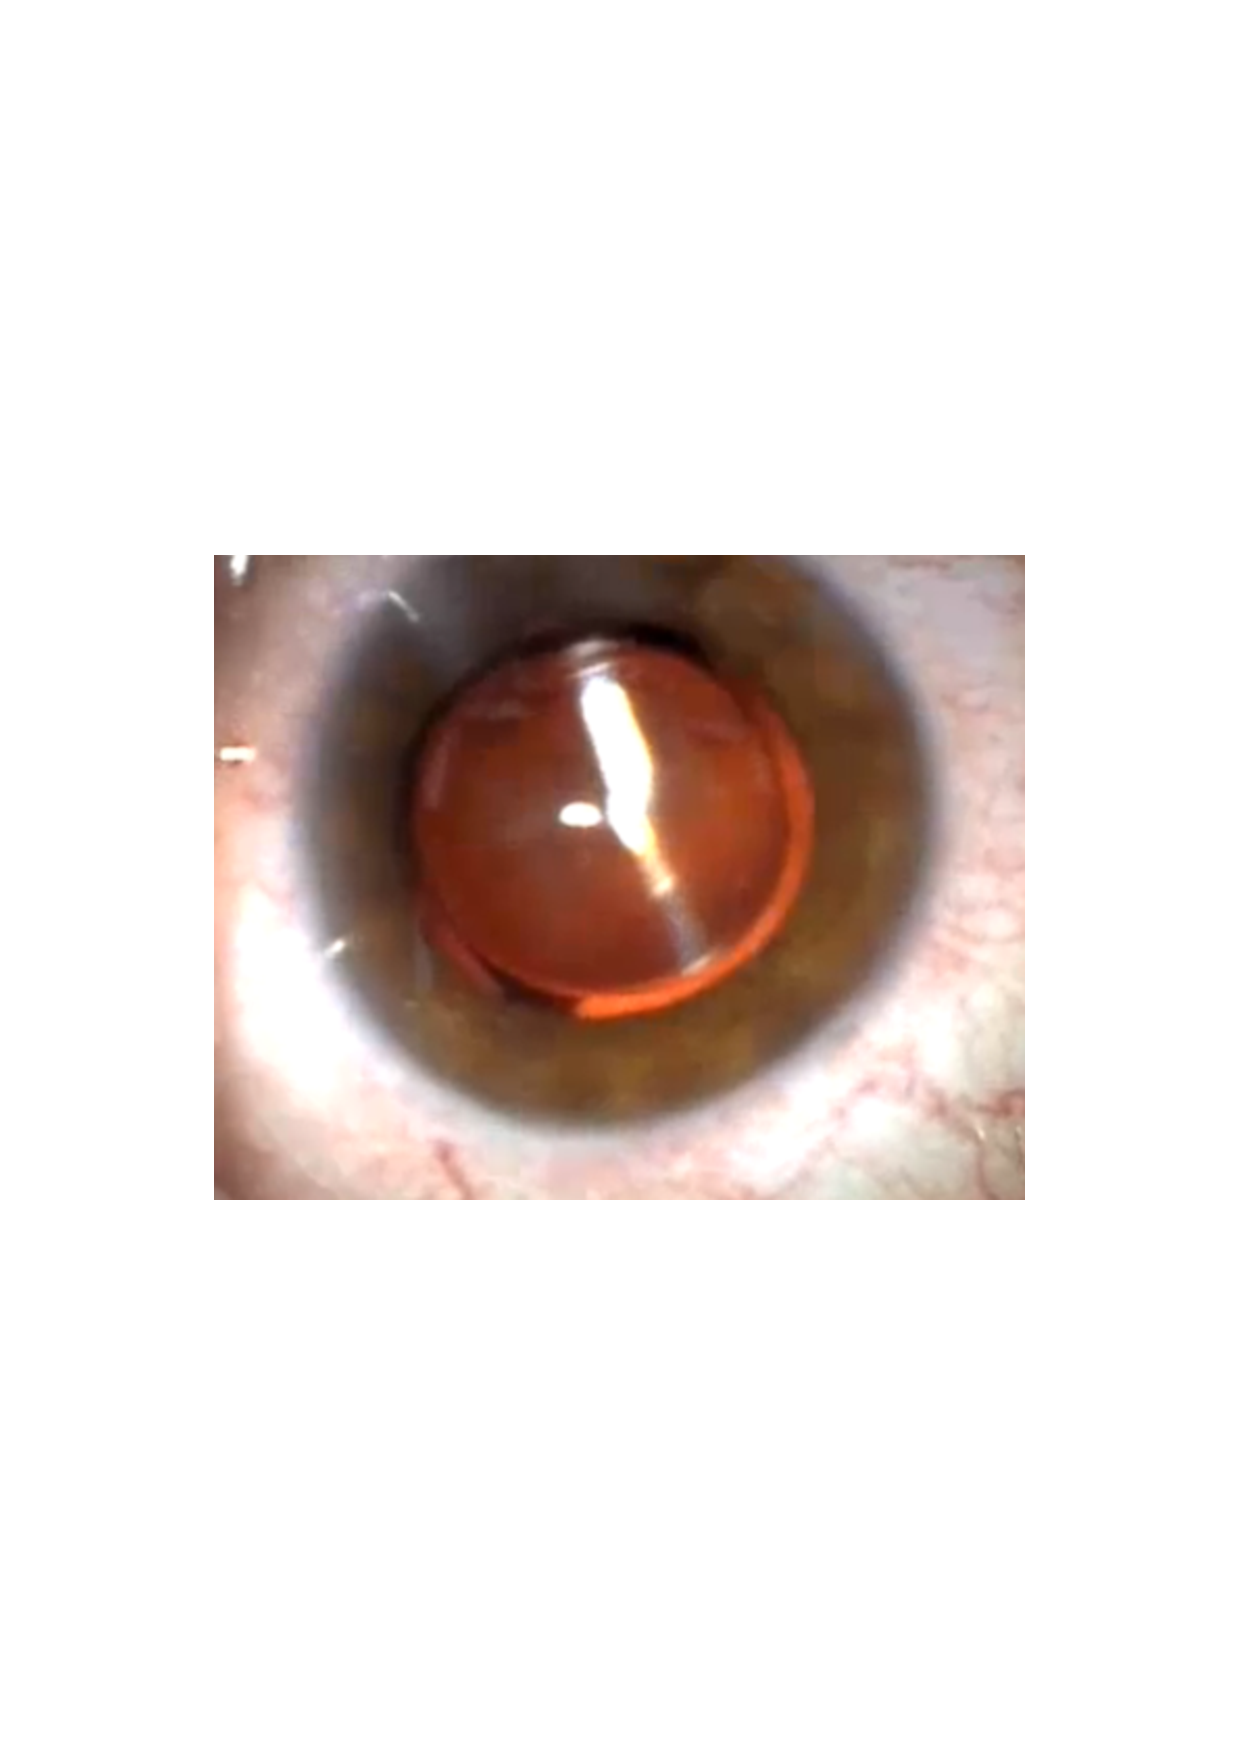
\includegraphics[width=4.5cm]{chapter9/surgery3.pdf} \\
\vspace{0.1cm}
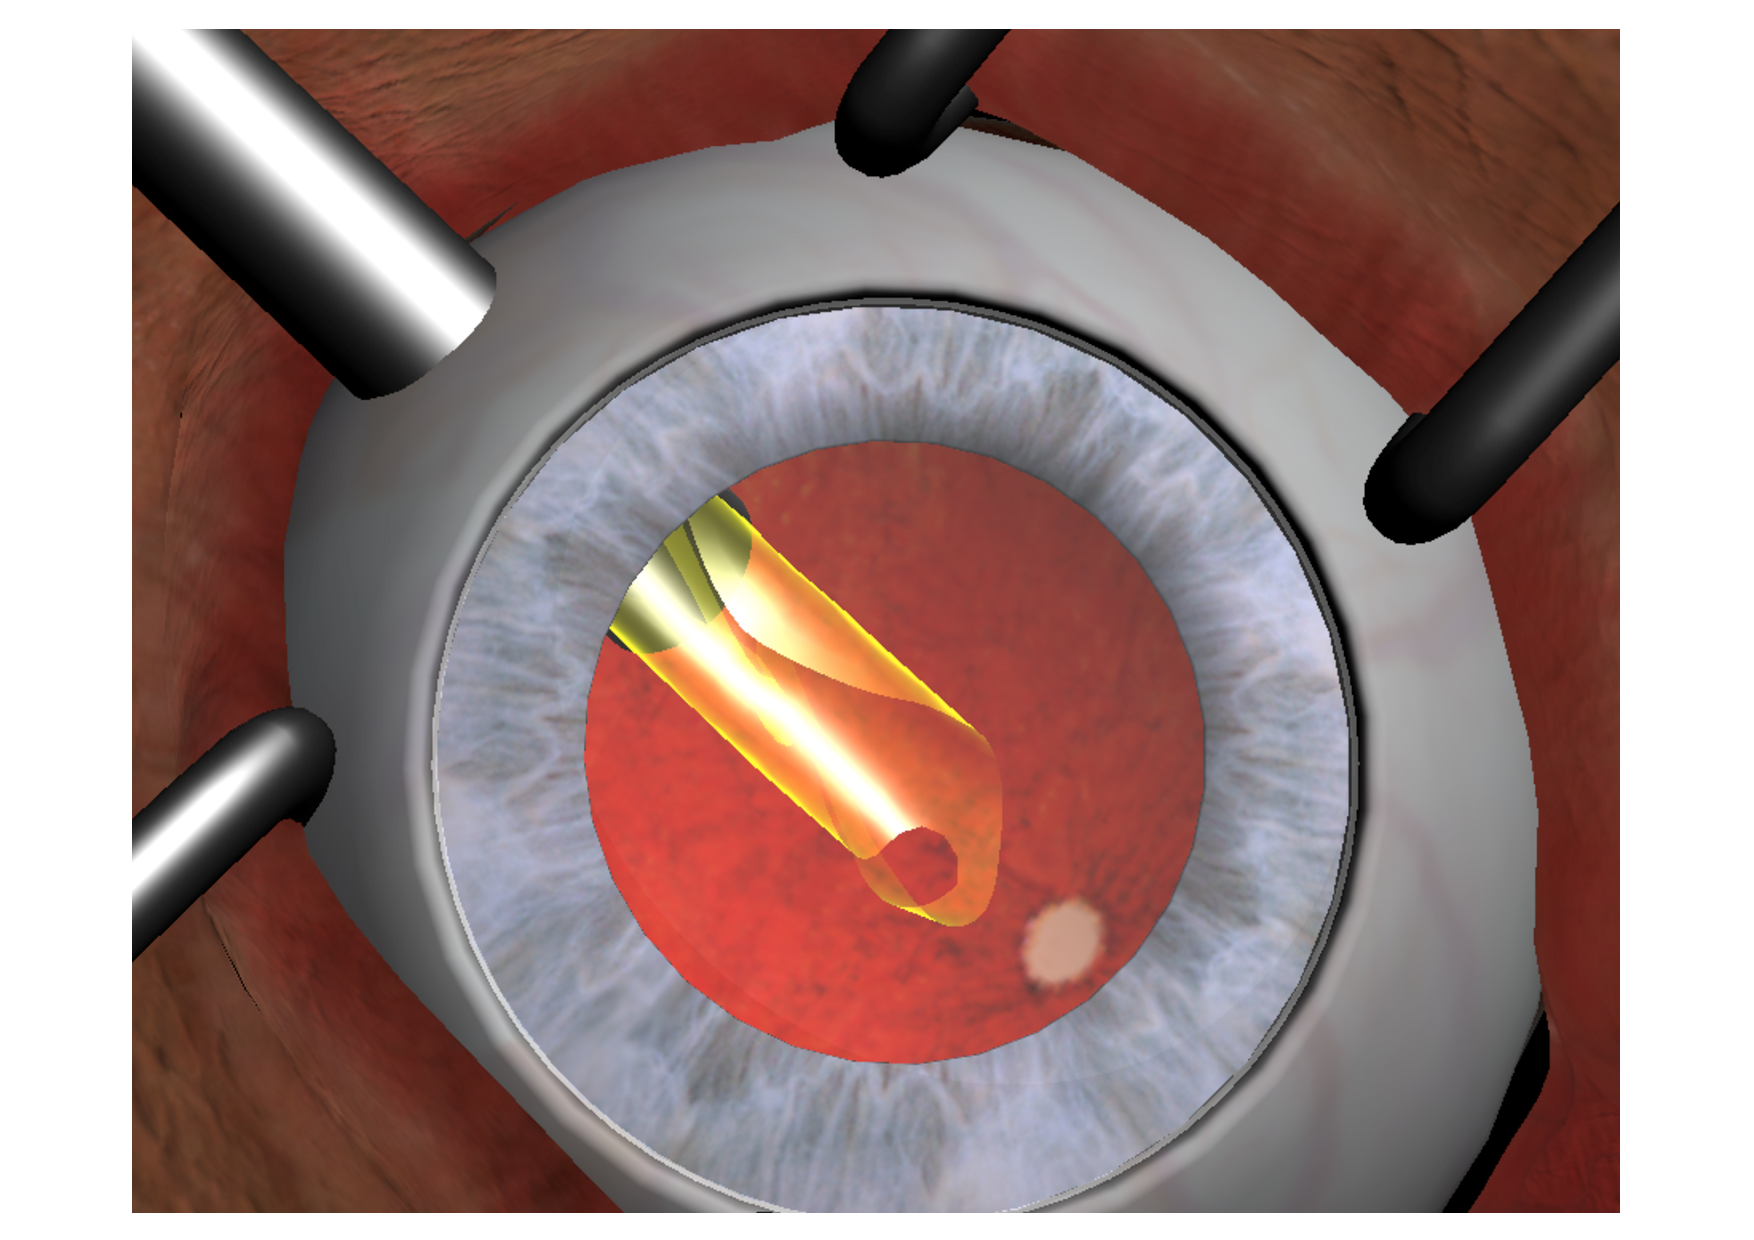
\includegraphics[width=4.5cm]{chapter9/simu1.pdf}
\hfill
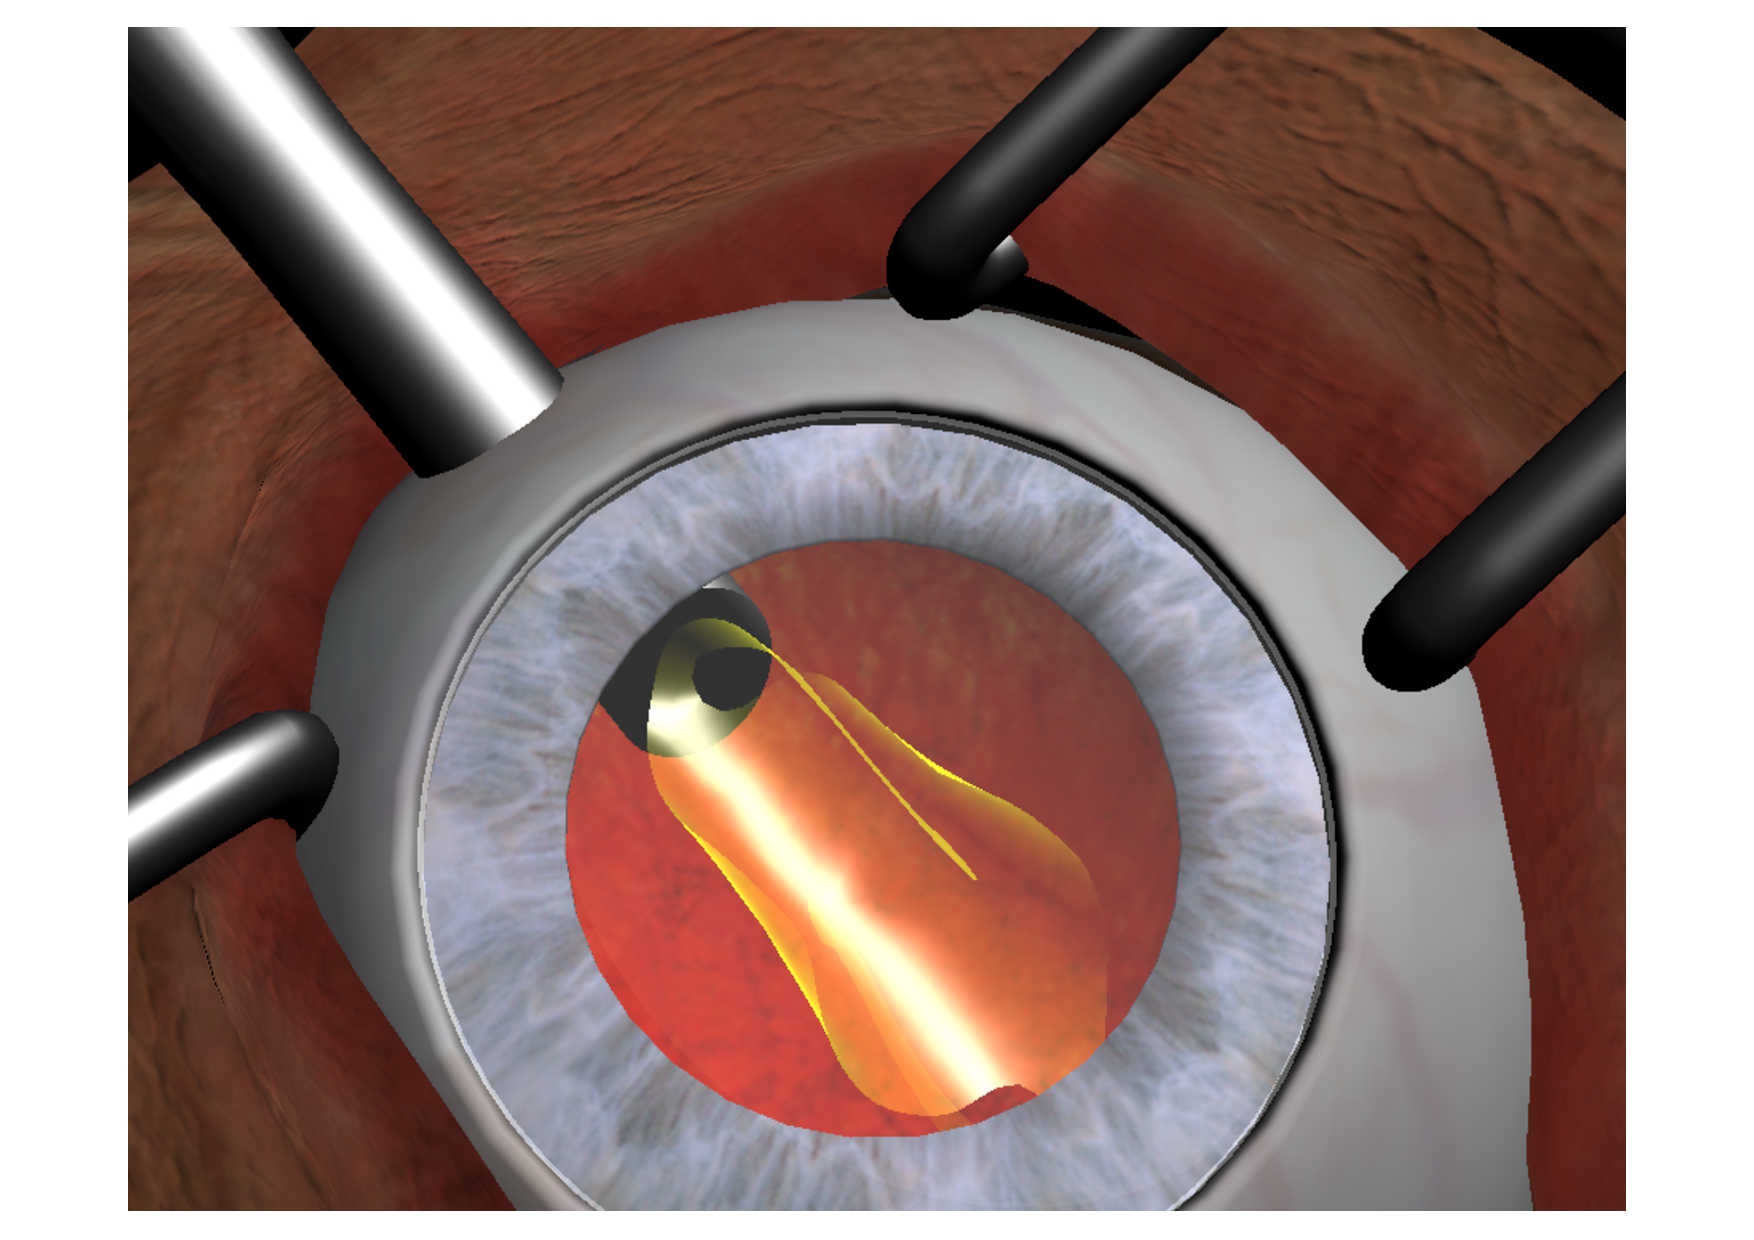
\includegraphics[width=4.5cm]{chapter9/simu2.pdf}
\hfill
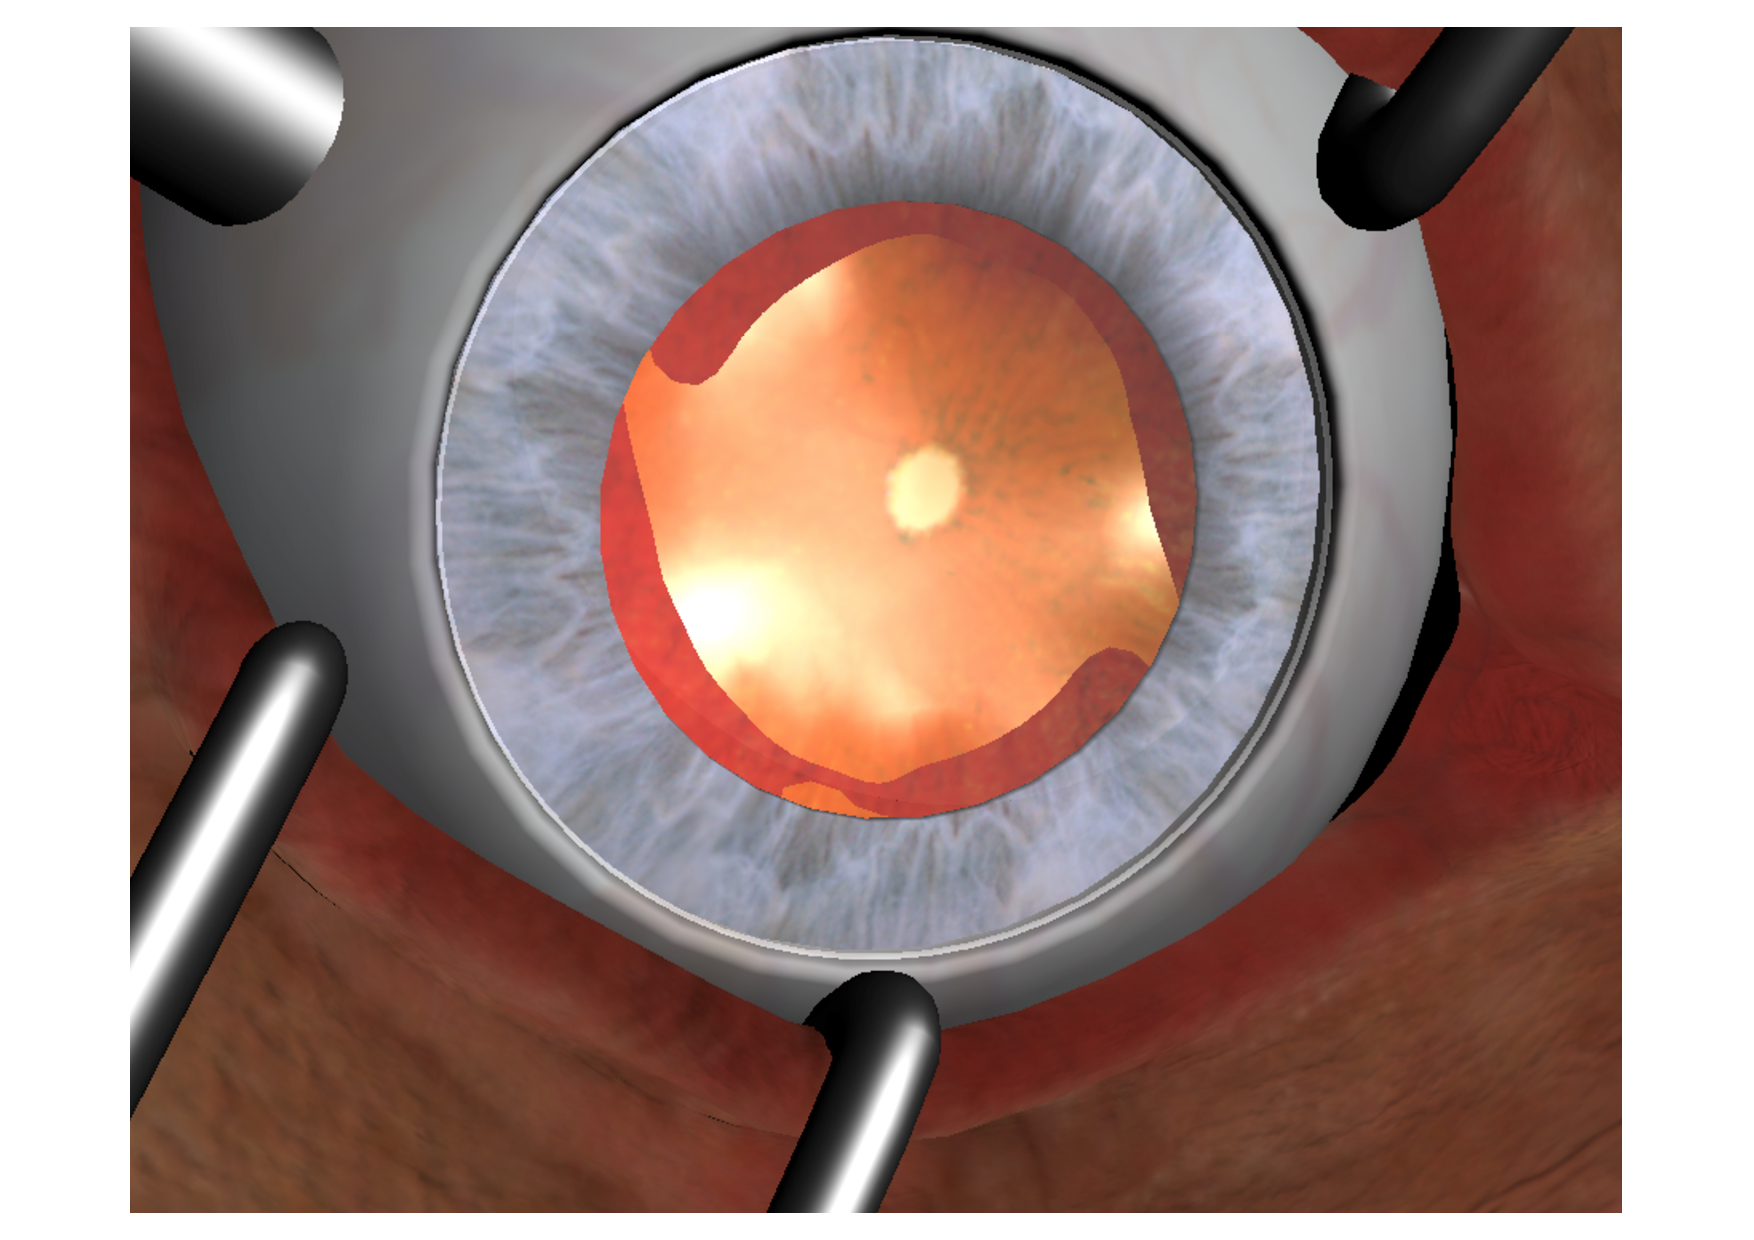
\includegraphics[width=4.5cm]{chapter9/simu3.pdf}
\caption [Lens imlant] {Three steps of the simulation of the intra-ocular lens implant injection and its deployment within the lens capsule. Top: images from a real cataract surgery, courtesy of Dr. Tarek Youssef, ophthalmologist in Canada. Below: our simulation of the implant's deployment.}
\label{chap9:fig-simu-results}
\end{figure}


\section{Discussion}

The finite element procedure that we propose was largely developed based on physical understanding without the use of mathematical shell theories. Indeed, our shell FEM was obtained by simply superimposing a plane stress and bending energies. According to \cite{Chapelle03}, this type of approach has a limited level of accuracy. The effective study of shell structures clearly requires a deep physical understanding of shell structural behaviours. The complexity of the physical behaviours of shells requires advanced mathematical analyses from theories that are still in development. The interested reader may refer to the book of \cite{Chapelle03} for more details on shell theory. If the range of application of our shell formulation might be somewhat limited, we did not find out any inconsistencies through our tests. We also need to keep in mind that the accuracy required in medical simulation is not the same than the one demanded in structural analyses for instance. Moreover, the additional complexity of a shell finite element formulation based on true shell theory may also very well jeopardise our real-time constraints. Therefore, we do not think that the use of this simple shell formulation significantly diminishes our contribution to the field of medical simulation. Indeed, to our knowledge, our co-rotational shell FEM is the first description of a shell finite element model applied to simulating the deformation of thin anatomical structures. 

Nevertheless, a few improvements are conceivable. Large strain could be allowed by using a non-linear strain tensor and more complex material laws (non-linear, viscoelasticity, etc.) could also be added to our shell formulation. However, those changes are substantial and their implementations are not straightforward. In addition, it is not clear how the benefits would be the greatest: whether from enhancing our model to a non-linear formulation or completely changing to another model based on true shell theory (where membrane and bending energies are not separated). The answer may depend on the type of constraints applied on the object. Also (as already mentioned section \ref{chap9:GPU}), the real-time capacity of our algorithm could be further improved by implementing our shell FEM on GPU. Although an optimal parallel re-implementation is always challenging, we have already reviewed why there was no major obstacle to a GPU implementation. 

\section{Conclusion}

We proposed a co-rotational formulation for shell elements by extending a classical in-plane triangular finite element approach. This simple shell element can efficiently handle both membrane, bending and twist forces. The validity of our approach has been demonstrated though comparison with theoretical results. It was then applied it to a rather complex application: the simulation of intra-ocular lens implant deployment in a cataract surgery simulation. These results are very encouraging and show the potential of such models. Examples include the modelling of hollow anatomical structures (colon, stomach, etc.), the simulation of cardiac valve leaflets, and blood vessels. This work on this co-rotational shell FEM formulation was the object of one main publications \citep{Comas2010a}.

So far, the mesh of the implant used in the cataract surgery simulation was created manually. However, manually creating the mesh is not suitable if we want to model the deformation of complex anatomical structures using shell elements. Therefore, the first step is to describe the surface of the structure that we want to simulate with curved patches. The goal is to create a mesh featuring the optimal number of curved shell elements while staying as close as possible to our targeted geometry. The following chapter deals with this problem. 
